\documentclass{prip}

\begin{document}

\predmet{Matematika}
\razred{1.~letnik}
\ucitelj{Jan Kastelic}
\sola{Splošna gimnazija}

%% 1 Osnove logike in teorije množic


%% 2 Naravna in cela števila


%% 3 Potence in izrazi


%% 4 Deljivost


%% 5 Racionalna števila
\begin{priprava}{0}{}{}{Racionalna števila}{}{}
    
    \chapter{Racionalna števila}

    \Large{Pregled vsebine poglavja in predvidenega števila ur:}

    \begin{table}[H]
        \centering
        \begin{tabular}{||c|c||} 
        \hhline{|t:==:t|}
        \rowcolor[rgb]{0.843,0.718,0.718} 
        Tema  & Predvideno število ur   \\ 
        \hhline{|:==:|}
        Racionalna števila & $1$    \\ 
        \hline
        Razširjanje in krajšanje ulomkov & $2$    \\ 
        \hline
        Računanje z ulomki & $3$    \\ 
        \hline
        Urejenost racionalnih števil & $1$     \\
        \hline
        Potence s celimi eksponenti & $3$     \\
        \hline
        Decimalni zapis & $1$    \\ 
        \hhline{|:==:|}
        Skupaj & $11$     \\
        \hhline{|b:==:b|}
        \end{tabular}
    \end{table}


    
\end{priprava}
\begin{priprava}{1}{}{Ulomki in racionalna števila}{Racionalna števila}{frontalna}{drsnice, projekcija, tabla}

    \section{Ulomki in racionalna števila}

        
            
                \textbf{Ulomek} $\dfrac{x}{y}$ je zapis, ki predstavlja zapis deljenja 
                $$x:y=\dfrac{x}{y};\quad y\neq 0\land x,y\in\mathbb{Z}.$$
                Število/izraz $x$ imenujemo \textbf{števec}, $y$ pa \textbf{imenovalec}, med njima je \textbf{ulomkova črta}.
            
                ~
            
                Ulomek $\dfrac{x}{0}$ ni definiran (nima pomena), saj z $0$ ne moremo deliti.
            
                ~
            
                \textbf{Algebrski ulomek} je ulomek, v katerem v števcu in/ali imenovalcu nastopajo algebrski izrazi.
            
                ~
            
                Vsako celo število $x\in\mathbb{Z}$ lahko zapišemo z ulomkom: $x=\dfrac{x}{1}$.
            
                ~
            
                \textbf{Ničelni ulomek} je ulomek oblike $\dfrac{0}{y}=0; y\neq 0$.
            
                ~
            
                V ulomku, kjer v števcu ali imenovalcu nastopa negativno število, upoštevamo enakost 
                $$-\dfrac{x}{y}=\dfrac{-x}{y}=\dfrac{x}{-y}.$$
            
                ~
            
                Vsakemu neničelnemu ulomku $\dfrac{x}{y}$ lahko priredimo njegovo \textbf{obratno vrednost}:
                $$\left(\dfrac{x}{y}\right)^{-1}=\dfrac{y}{x}; \quad x,y\in\mathbb{Z}\setminus\{0\}.$$
            

        


        
            \subsection*{Racionalna števila}

            
                Množica racionalnih števil $\mathbb{Q}$ je sestavljena iz vseh ulomkov (kar pomeni, da vsebuje tudi vsa naravna in cela števila).

                $$\mathbb{Q}=\left\{\frac{x}{y}; \ x\in\mathbb{Z}, y\in\mathbb{Z}\setminus\{0\}\right\}$$
            
                \begin{figure}[H]
                \centering
                \begin{tikzpicture}
                    % \clip (0,0) rectangle (14.000000,10.000000);
                    {\footnotesize
                    
                    % Drawing segment A B
                    \draw [line width=0.016cm] (1.000000,1.500000) -- (4.460000,1.500000);%
                    \draw [line width=0.016cm] (4.540000,1.500000) -- (8.000000,1.500000);%
                    
                    % Marking point 0 by circle
                    \draw [line width=0.016cm] (4.500000,1.500000) circle (0.040000);%
                    \draw (4.500000,1.500000) node [anchor=south] { $0$ };%
                    
                    
                    % Changing color 255 0 0
                    \definecolor{r255g0b0}{rgb}{1.000000,0.000000,0.000000}%
                    \color{r255g0b0}% 
                    
                    % Marking point \mathbb{Q}^+
                    \draw (6.250000,1.500000) node [anchor=south] { $\mathbb{Q}^+$ };%
                    
                    % Drawing segment B 0
                    \draw [line width=0.016cm] (8.000000,1.500000) -- (4.540000,1.500000);%
                    }

                    
                    % Changing color 0 255 0
                    \definecolor{r0g255b0}{rgb}{0.000000,1.000000,0.000000}%
                    \color{r0g255b0}% 
                    
                    % Marking point \mathbb{Q}^-
                    \draw (2.750000,1.500000) node [anchor=south] { $\mathbb{Q}^-$ };%
                    
                    % Drawing segment A 0
                    \draw [line width=0.016cm] (1.000000,1.500000) -- (4.460000,1.500000);%
                    

                    % Changing color 0 0 0
                    \definecolor{r0g0b0}{rgb}{0.000000,0.000000,0.000000}%
                    \color{r0g0b0}% 
                    
                    % Marking point \mathbb{Q}
                    \draw (1.500000,2.000000) node  { $\mathbb{Q}$ };%
                    \color{black}
                    
                    \end{tikzpicture}
                \end{figure}
                    
            

            
                Glede na predznak razdelimo racionalna števila v tri množice:
                \begin{itemize}
                    \item \textcolor{green}{množico negativnih racionalnih števil $\mathbf{\mathbb{Q}^-}$},
                    \item množico z elementom nič: $\mathbf{\{0\}}$ in
                    \item \textcolor{red}{množico pozitivnih racionalnih števil: $\mathbf{\mathbb{Q}^+}$}.
                \end{itemize}
                $$ \mathbb{Q}=\textcolor{green}{\mathbb{Q}^-}\cup\{0\}\cup\textcolor{red}{\mathbb{Q}^+} $$
            
            

            % 
            %     Množica racionalnih števil je povsod gosta, saj lahko med poljubnima racionalnima številoma vedno najdemo racionalno število (posledično je med dvema racionalnima številoma neskončno mnogo racionalnih števil).
            % 

        

        
            
                Ulomka $\dfrac{x}{y}$ in $\dfrac{w}{z}$ sta enaka/enakovredna natanko takrat, ko je $xz=wy$; $y,z\neq 0$.
                $$\dfrac{x}{y}=\dfrac{w}{z}\Leftrightarrow xz=wy; \quad y,z\neq 0$$
            

            
                Enaka/enakovredna ulomka sta različna zapisa za isto racionalno število.
            
        ~\\



%%% naloge

        \begin{multicols}{2}

            \begin{naloga}
                Za katere vrednosti $x$ ulomek ni definiran?
                \begin{itemize}
                    \item $\frac{x-2}{x+1}$ 
                    \item $\frac{2}{x-5}$ 
                    \item $\frac{x+2}{3}$ 
                    \item $\frac{13}{2x-5}$ 
                \end{itemize}
            \end{naloga}
        

        
            \begin{naloga}
                Za katere vrednosti $x$ ima ulomek vrednost enako $0$?
                \begin{itemize}
                    \item $\frac{x-2}{x+1}$ 
                    \item $\frac{2}{x-5}$ 
                    \item $\frac{x+2}{3}$ 
                    \item $\frac{13}{2x-5}$ 
                \end{itemize}
            \end{naloga}
        

        
            \begin{naloga}
                Ali imata ulomka isto vrednost?
                \begin{itemize}
                    \item $\frac{2}{3}$ in $\frac{10}{15}$ 
                    \item $\frac{-1}{2}$ in $\frac{1}{-2}$ 
                    \item $\frac{4}{5}$ in $\frac{-8}{-10}$ 
                    \item $\frac{5}{8}$ in $\frac{8}{5}$ 
                \end{itemize}
            \end{naloga}
        

        
            \begin{naloga}
                Za kateri $x$ imata ulomka isto vrednost?
                \begin{itemize}
                    \item $\frac{x+1}{2}$ in $\frac{3}{4}$ 
                    \item $\frac{4}{2x-1}$ in $\frac{1}{3}$ 
                    \item $\frac{x+1}{2}$ in $\frac{x-1}{-3}$ 
                    \item $\frac{x+1}{x-2}$ in $\frac{2}{5}$ 
                \end{itemize}
            \end{naloga}
        

        
            \begin{naloga}
                Ali ulomka predstavljata isto vrednost?
                \begin{itemize}
                    \item $\left(\frac{1}{2}\right)^{-1}$ in $-\frac{1}{2}$ 
                    \item $\left(\frac{2}{3}\right)^{-1}$ in $\frac{3}{2}$ 
                    \item $ 1\frac{3}{7}$ in $\left(\frac{7}{10}\right)^{-1}$ 
               \end{itemize}
            \end{naloga}
        

        
            \begin{naloga}
                Ali ulomka predstavljata isto vrednost?
                \begin{itemize}
                    \item $ 2\cdot\frac{3}{4}$ in $\frac{3}{2}$ 
                    \item $ 2\frac{3}{4}$ in $\frac{3}{2}$ 
                    \item $\left(1\frac{2}{5}\right)^{-1}$ in $ 1\frac{5}{2}$ 
                    \item $\left(1\frac{2}{5}\right)^{-1}$ in $\frac{5}{7}$ 
               \end{itemize}
            \end{naloga}
        

        
            \begin{naloga}
                Zapišite s celim delom oziroma z ulomkom.
                \begin{itemize}
                            \item $\frac{14}{5}$ 
                            \item $-\frac{5}{2}$ 
                            \item $\frac{4}{3}$ 
                            \item $\frac{110}{17}$ 
                            \item $ 3\frac{5}{8}$ 
                            \item $ 2\frac{9}{2}$                  
               \end{itemize}
            \end{naloga}
            ~\\~~\\

        \end{multicols}
        


\end{priprava}
\begin{priprava}{2., 3}{}{Razširjanje in krajšanje ulomkov}{Racionalna števila}{frontalna}{drsnice, projekcija, tabla}

    \section{Razširjanje in krajšanje ulomkov}

        

            \subsection*{Razširjanje ulomka}
                Ulomek ohrani svojo vrednost, če števec in imenovalec pomnožimo z istim neničelnim številom oziroma izrazom.
                Temu postopku pravimo \textbf{razširjanje ulomka}.

                $$\dfrac{x}{y}=\dfrac{x\cdot z}{y\cdot z}; \quad x\in\mathbb{Z} \land y,z\in\mathbb{Z}\setminus\{0\}$$
            

            
                Ko ulomke seštevamo ali odštevamo, jih razširimo na \textbf{najmanjši skupni imenovalec}, 
                ki je najmanjši skupni večkratnik vseh imenovalcev.
            

        

        
            \subsection*{Krajšanje ulomka}
                Vrednost ulomka se ne spremeni, če števec in imenovalec delimo z istim neničelnim številom oziroma izrazom.
                Temu postopku rečemo \textbf{krajšanje ulomka}.

                $$\dfrac{x\cdot z}{y\cdot z}=\dfrac{x}{y}; \quad x\in\mathbb{Z}\land y,z\in\mathbb{Z}\setminus\{0\} $$
            
                ~

                Ulomek $\dfrac{x}{y}$ je \textbf{okrajšan}, če je $(x,y)=1$, torej če sta števec in imenovalec tuji števili.
            
        
            ~\\

        %%% naloge

        \begin{multicols}{2}

        
            \begin{naloga}
                Razširite ulomke na najmanjši skupni imenovalec.
                \begin{itemize}
                            \item $\frac{1}{3}$, $\frac{3}{5}$ in $\frac{5}{6}$ 
                            \item $\frac{2}{7}$, $1$ in $\dfrac{1}{2}$ 
                            \item $\frac{5}{6}$, $\frac{1}{2}$ in $-\frac{2}{3}$ 
                            \item $\frac{1}{5}$, $-\frac{1}{2}$ in $\frac{-1}{3}$ 
                            \item $\frac{2}{-1}$, $\frac{3}{2}$ in $\frac{1}{-3}$ 
                            \item $\frac{3}{-4}$, $\frac{-1}{2}$ in $-\frac{2}{5}$ 
                \end{itemize}
            \end{naloga}
        

        
            \begin{naloga}
                Razširite ulomke na najmanjši skupni imenovalec.
                \begin{itemize}
                            \item $\frac{1}{x-1}$, $\frac{1}{x+1}$ in $1$ 
                            \item $\frac{2}{x}$, $\frac{1}{x-3}$ in $\frac{1}{(x-3)^2}$ 
                            \item $\frac{3}{x^2-4x}$, $\frac{1}{x}$ in $\frac{2}{x-4}$ 
                            \item $\frac{4}{x-4}$, $\frac{2}{x-2}$ in $\frac{1}{x^2-6x+8}$ 
                            \item $\frac{2}{x-1}$ in $\frac{3}{1-x}$ 
                            \item $\frac{1}{2-x}$, $\frac{2}{x+2}$ in $\frac{3}{x^2-4}$ 
                \end{itemize}
            \end{naloga}
        

        
            \begin{naloga}
                Okrajšajte ulomek.
                \begin{itemize}
                    \item $\frac{100}{225}$ 
                    \item $\frac{34}{51}$ 
                    \item $\frac{121}{3}$ 
                    \item $\frac{45}{75}$ 
                \end{itemize}
            \end{naloga}
        

        
            \begin{naloga}
                Okrajšajte ulomek.
                \begin{itemize}
                            \item $\frac{x^2-4}{x^2+2x}$ 
                            \item $\frac{x^3+8}{2x+4}$ 
                            \item $\frac{x^3-1}{x^2-4x+3}$ 
                            \item $\frac{x^3-2x^2-x+2}{x^2-3x+2}$ 
                            \item $\frac{x^2-9}{3-x}$ 
                            \item $\frac{x-4}{16-x^2}$ 
                \end{itemize}
            \end{naloga}
        
            ~\\~\\
        \end{multicols}

\end{priprava}
\begin{priprava}{4., 5., 6}{}{Računanje z ulomki}{Racionalna števila}{frontalna}{drsnice, projekcija, tabla}

    \section{Seštevanje in odštevanje ulomkov}

        
    \subsection*{Seštevanje ulomkov}
        Ulomke \textbf{seštevamo} tako, da jih razširimo na skupni imenovalec, nato seštejemo števce, imenovalce pa prepišemo.
        $$\dfrac{x}{y}+\dfrac{z}{w}=\dfrac{xw}{yw}+\dfrac{yz}{yw}=\dfrac{xw+yz}{yw}; \quad x,z\in\mathbb{Z}\land y,w\in\mathbb{Z}\setminus\{0\} $$
    

    \subsection*{Odštevanje ulomkov}
        Ulomke \textbf{odštevamo} tako, da prištejemo nasprotni ulomek.
        $$\dfrac{x}{y}-\dfrac{z}{w}=\dfrac{x}{y}+\left(-\dfrac{z}{w}\right)=\dfrac{xw}{yw}+\dfrac{-yz}{yw}=\dfrac{xw-yz}{yw}; \quad x,z\in\mathbb{Z}\land y,w\in\mathbb{Z}\setminus\{0\} $$
    



    ~\\

%%% naloge

    \begin{naloga}
        Izračunajte.
        \begin{itemize}
            \item $\frac{5}{7}+\frac{1}{14}$ 
            \item $\frac{2}{9}-\frac{1}{3}$ 
            \item $\frac{3}{8}+1\frac{1}{2}$ 
            \item $1-\frac{5}{6}$ 
        \end{itemize}
    \end{naloga}



    \begin{naloga}
        Izračunajte.
        \begin{itemize}
            \item $\left(\frac{2}{3}-2\frac{1}{4}\right)+\frac{1}{12}$ 
            \item $\frac{2}{7}-\frac{3}{4}+\left(\frac{1}{2}-2\right)$ 
            \item $\left(\frac{2}{3}-\left(\frac{1}{3}-3\right)+\frac{1}{4}\right)-\frac{1}{2}$ 
            \item $1-\left(2-\left(3-4-\left(5-\frac{1}{2}\right)\right)+\frac{1}{3}\right)$ 
        \end{itemize}
    \end{naloga}




    \begin{naloga}
        Poenostavite.
        \begin{itemize}
            \item $\frac{x}{x-1}-\frac{x}{x+1}$ 
            \item $\frac{3}{x^2}+\frac{4}{x^3}-\frac{1}{x}$ 
            \item $\frac{3}{x^2-4x}-\left(\frac{1}{x-4}+\frac{2}{x^2-5x+4}\right)$ 
            \item $\frac{2}{xy}+\frac{3}{x}-\frac{2}{y}$ 
        \end{itemize}
    \end{naloga}




    \begin{naloga}
        Poenostavite.
        \begin{itemize}
            \item $\frac{(x-3)^2+(x+3)^2}{x^2+9}-\frac{3x^2}{2x^2-x^2}$ 
            \item $\frac{(a-3)^3-(a-1)^3+26}{6a}+\left(-\frac{1}{2}\right)^{-1}$ 
            \item $\frac{x^3-2x^2-x+2}{-x(1-x)-2}-\left(\frac{x-1}{x}-1\right)^{-1}$ 
            \item $\left(\frac{x}{2}-\left(\frac{x}{3}-\left(\frac{x}{4}-\frac{x}{5}\right)\right)\right)-\left(\frac{60}{x}\right)^{-1}$ 
        \end{itemize}
    \end{naloga}


    ~
%%% Množenje ulomkov

\section{Množenje ulomkov}


        Ulomka \textbf{množimo} tako, da števce množimo s števci, imenovalce pa množimo z imenovalci.
        $$\dfrac{x}{y}\cdot \dfrac{z}{w}=\dfrac{xz}{yw}; \quad x,z\in\mathbb{Z}\land y,w\in\mathbb{Z}\setminus\{0\}$$
        
    
        Produkt danega in njemu obratnega ulomka je enak $1$.
        $$\dfrac{x}{y}\cdot\left(\dfrac{x}{y}\right)^{-1}=\dfrac{x}{y}\cdot\dfrac{y}{x}=1$$
    

    ~
%%% naloge


    \begin{naloga}
        Izračunajte.
        \begin{itemize}
                    \item $\frac{1}{3}\cdot \frac{3}{7}$ 
                    \item $\frac{-2}{13}\cdot \left(-\frac{39}{4}\right)$ 
                    \item $\frac{2}{5}\cdot \frac{4}{9}$ 
                    \item $2\frac{1}{3}\cdot 3\frac{3}{4}$ 
                    \item $\frac{-2}{5}\cdot 4\frac{2}{7}$ 
                    \item $3\cdot\frac{2}{3}$ 
        \end{itemize}
    \end{naloga}




    \begin{naloga}
        Poenostavite.
        \begin{itemize}
            \item $\frac{x^2-9}{x^2+3x+9}\cdot\frac{x^3-27}{x^2-6x+9}$ 
            \item $\frac{x^2+5x}{-x+2}\cdot\frac{2x^2-8}{x^2+7x+10}$ 
            \item $\frac{x^3-4x^2-4x+16}{2x+4}\cdot\frac{6x}{3x-6}$ 
            \item $2\cdot\frac{x}{x-1}\cdot\frac{x^2-1}{x^2+x}$ 
        \end{itemize}
    \end{naloga}




    \begin{naloga}
        Poenostavite.
        \begin{itemize}
            \item $\frac{x^2-4}{x^2-1}\cdot\frac{x^3-1}{x^3+x^2+x}\cdot\frac{x^2+x}{2-x}$ 
            \item $\left(\frac{6-x}{x^2+6x}-\frac{x}{36-x^2}\right)\cdot\left(\frac{2x-6}{x^2+6x}\right)^{-1}+\frac{x}{6-x}$ 
            \item $\left(\left(x-y+\left(\frac{x+y}{2xy}\right)^{-1}\right)\cdot\left(\frac{1}{x+y}\right)^{-1}-2xy\right)\cdot(x-y)^{-1}$ 
            \item $\left(xy+y^2-\frac{xy+y^2}{3xy-3x^2}\right)\cdot\left(\frac{x+y}{3x}\right)^{-1}-\left(-\frac{y-x}{y}\right)^{-1}$ 
        \end{itemize}
    \end{naloga}



    ~
%%% Deljenje ulomkov

\section{Deljenje ulomkov}


        Ulomek \textbf{delimo} z neničelnim ulomkom tako, da prvi ulomek množimo z obratno vrednostjo drugega ulomka.
        $$\dfrac{x}{y}:\dfrac{z}{w}=\dfrac{x}{y}\cdot\left(\dfrac{z}{w}\right)^{-1}=\dfrac{x}{y}\cdot\dfrac{w}{z}=\dfrac{xw}{yz}; \quad x\in\mathbb{Z}\land y,z,w\in\mathbb{Z}\setminus\{0\} $$
    

    
        Deljenje ulomkov lahko zapišemo kot \textbf{dvojni ulomek}.
        $$\dfrac{x}{y}:\dfrac{z}{w}=\dfrac{\frac{x}{y}}{\frac{z}{w}}; \quad x\in\mathbb{Z}\land y,z,w\in\mathbb{Z}\setminus\{0\} $$
    

        ~



%%% naloge


    \begin{naloga}
        Izračunajte.
        \begin{itemize}
            \item $2:\frac{4}{5}$ 
            \item $1\frac{2}{3}:2\frac{5}{6}$ 
            \item $\frac{7}{12}:14$ 
            \item $\frac{3}{8}:\frac{9}{32}$ 
        \end{itemize}
    \end{naloga}




    \begin{naloga}
        Izračunajte.
        \begin{itemize}
                    \item $\dfrac{\frac{3}{4}}{\frac{6}{8}}$ 
                    \item $\dfrac{\frac{1}{2}}{2}$ 
                    \item $\dfrac{3}{\frac{5}{6}}$ 
                    \item $\dfrac{\frac{2}{-5}}{\frac{-1}{5}}$ 
                    \item $\dfrac{\frac{3}{5}}{-2}$ 
                    \item $\dfrac{-\frac{1}{2}}{2^{-1}}$ 

        \end{itemize}
    \end{naloga}




    \begin{naloga}
        Poenostavite.
        \begin{itemize}
            \item $\frac{x^2+x-6}{x+2}:(x-2)$ 
            \item $\frac{x-1}{2x^2-4x}:\frac{x^2}{x-2}$ 
            \item $x:\frac{x^2+x}{x^3+1}$ 
        \end{itemize}
    \end{naloga}



    \begin{naloga}
        Poenostavite.
        \begin{itemize}
            \item $\frac{x-1}{x^2-4}:\frac{1-x^2}{x-2}$ 
            \item $\frac{x-2}{(x+2)^{-1}}:\left(\frac{1}{x^2-1}\right)^{-1}$ 
            \item $\frac{3-x}{2-x}:\frac{x-3}{x-2}$ 
        \end{itemize}
    \end{naloga}



\end{priprava}
\begin{priprava}{7}{}{Urejenost racionalnih števil}{Racionalna števila}{frontalna}{drsnice, projekcija, tabla}

    \section{Urejenost racionalnih števil}

            
    
    Za ulomka $\dfrac{x}{y}$ in $\dfrac{z}{w}$ ($y,w\notin\{0\}$) velja natanko ena izmed treh možnosti:
    
    \begin{enumerate}
        \item prvi ulomek je večji od drugega $\dfrac{x}{y}\geq\dfrac{z}{w}$ natanko tedaj, ko je $xw\geq yz$;
        \item drugi ulomek je večji od prvega $\dfrac{x}{y}\leq\dfrac{z}{w}$ natanko tedaj, ko je $xw\leq yz$;
        \item ulomka sta enaka $\dfrac{x}{y}=\dfrac{z}{w}$ natanko tedaj, ko je $xw=yz$ oziroma $\dfrac{x}{y}\leq\dfrac{z}{w} \land \dfrac{x}{y}\geq\dfrac{z}{w}$.
    \end{enumerate}


    Enaka ulomka predstavljata isto racionalno število.

    ~

    Slika večjega racionalnega števila \textcolor{red}{$\dfrac{x}{y}$} je na številski premici desno od slike manjšega racionalnega števila \textcolor{green}{$\dfrac{z}{w}$}.
\begin{figure}[H]
    \centering
    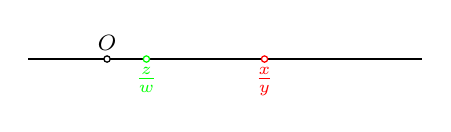
\begin{tikzpicture}
        % \clip (0,0) rectangle (14.000000,10.000000);
        {\footnotesize
        
        % Drawing segment A B
        \draw [line width=0.016cm] (1.000000,1.500000) -- (1.960000,1.500000);%
        \draw [line width=0.016cm] (2.040000,1.500000) -- (2.460000,1.500000);%
        \draw [line width=0.016cm] (2.540000,1.500000) -- (3.960000,1.500000);%
        \draw [line width=0.016cm] (4.040000,1.500000) -- (6.000000,1.500000);%
        
        % Marking point O by circle
        \draw [line width=0.016cm] (2.000000,1.500000) circle (0.040000);%
        \draw (2.000000,1.500000) node [anchor=south] { $O$ };%
        
        % Changing color 255 0 0
        \definecolor{r255g0b0}{rgb}{1.000000,0.000000,0.000000}%
        \color{r255g0b0}% 
        
        % Marking point \frac{x}{y} by circle
        \draw [line width=0.016cm] (4.000000,1.500000) circle (0.040000);%
        \draw (4.000000,1.500000) node [anchor=north] { $\frac{x}{y}$ };%
        
        % Changing color 0 255 0
        \definecolor{r0g255b0}{rgb}{0.000000,1.000000,0.000000}%
        \color{r0g255b0}% 
        
        % Marking point \frac{z}{w} by circle
        \draw [line width=0.016cm] (2.500000,1.500000) circle (0.040000);%
        \draw (2.500000,1.500000) node [anchor=north] { $\frac{z}{w}$ };%
        \color{black}
        }
    \end{tikzpicture}
\end{figure}    


Slike pozitivnih racionalnih števil ležijo desno, slike negativnih racionalnih števil pa levo od koordinatnega izhodišča.
    \begin{figure}[H]
        \centering
        \begin{tikzpicture}
            
            % \clip (0,0) rectangle (14.000000,10.000000);
            {\footnotesize
            
            % Drawing segment A B
            \draw [line width=0.016cm] (1.000000,1.500000) -- (3.460000,1.500000);%
            \draw [line width=0.016cm] (3.540000,1.500000) -- (6.000000,1.500000);%
            
            % Changing color 255 0 0
            \definecolor{r255g0b0}{rgb}{1.000000,0.000000,0.000000}%
            \color{r255g0b0}% 
            
            % Drawing segment B O
            \draw [line width=0.016cm] (6.000000,1.500000) -- (3.540000,1.500000);%
            
            % Marking point pozitivna_tevila
            \draw (4.750000,1.500000) node [anchor=north] { $pozitivna~ števila$ };%
            \draw (4.750000,1.500000) node [anchor=south] { $\mathbb{Q}^+$ };%
            
            % Changing color 0 255 0
            \definecolor{r0g255b0}{rgb}{0.000000,1.000000,0.000000}%
            \color{r0g255b0}% 
            
            % Drawing segment O A
            \draw [line width=0.016cm] (3.460000,1.500000) -- (1.000000,1.500000);%
            
            % Marking point negativna_tevila
            \draw (2.250000,1.500000) node [anchor=north] { $negativna~ števila$ };%
            \draw (2.250000,1.500000) node [anchor=south] { $\mathbb{Q}^-$ };%
            
            % Changing color 0 0 0
            \definecolor{r0g0b0}{rgb}{0.000000,0.000000,0.000000}%
            \color{r0g0b0}% 
            
            % Marking point O by circle
            \draw [line width=0.032cm] (3.500000,1.500000) circle (0.040000);%
            \draw (3.500000,1.500000) node [anchor=south] { $O$ };%
            \color{black}
            }
        \end{tikzpicture}
    \end{figure}

    

    V množici ulomkov velja, da je vsak negativen ulomek manjši od vsakega pozitivnega ulomka.


    ~

    Množica racionalnih števil je \textbf{linearno urejena} z relacijo \textit{biti manjši ali enak} ($\leq$) oziroma \textit{biti večji ali enak} ($\geq$). 
    
    Za to relacijo linearne urejenosti veljajo naslednje lastnosti:

    \begin{itemize}
        \item \textbf{refleksivnost}: $\forall \dfrac{x}{y}\in\mathbb{Q}: \dfrac{x}{y}\leq\dfrac{x}{y}$;
        \item \textbf{antisimetričnost}: $\forall \dfrac{x}{y},\dfrac{z}{w}\in\mathbb{Q}: \dfrac{x}{y}\leq\dfrac{z}{w}  \land \dfrac{z}{w}\leq\dfrac{x}{y} \Rightarrow \dfrac{x}{y}=\dfrac{z}{w}$;
        \item \textbf{tranzitivnost}: $\forall \dfrac{x}{y},\dfrac{z}{w},\dfrac{r}{q}\in\mathbb{Q}: \dfrac{x}{y}\leq\dfrac{z}{w}  \land \dfrac{z}{w}\leq\dfrac{r}{q} \Rightarrow \dfrac{x}{y}\leq\dfrac{r}{q}$ in 
        \item \textbf{stroga sovisnost}: $\forall \dfrac{x}{y},\dfrac{z}{w}\in\mathbb{Q}: \dfrac{x}{y}\leq\dfrac{z}{w}  \lor \dfrac{z}{w}\leq\dfrac{x}{y}$.
    \end{itemize}

~

    Množica racionalnih števil pa je tudi \textbf{delno urejena}, in sicer z relacijo \textit{biti manjši} ($<$) oziroma \textit{biti večji} ($>$). 

    Tedaj veljajo le lastnosti: \textbf{refleksivnost}, \textbf{antisimetričnost} in \textbf{tranzitivnost}.


    ~

    Pri množenju neenakosti s pozitivnim številom se znak neenakosti ohrani.
    $$ \dfrac{x}{y}<\dfrac{z}{w} \quad \wedge \quad \dfrac{r}{q}>0 \quad \Rightarrow \quad \dfrac{x}{y}\cdot\dfrac{r}{q}<\dfrac{z}{w}\cdot\dfrac{r}{q} $$

    

    Pri množenju neenakosti s negativnim številom se znak neenakosti obrne.
    $$ \dfrac{x}{y}<\dfrac{z}{w} \quad \wedge \quad \dfrac{r}{q}<0 \quad \Rightarrow \quad \dfrac{x}{y}\cdot\dfrac{r}{q}>\dfrac{z}{w}\cdot\dfrac{r}{q} $$


    \subsubsection*{Monotonost vsote}
    Če na obeh straneh neenakosti prištejemo isto število, se neenakost ohrani.
    $$ \dfrac{x}{y}<\dfrac{z}{w} \quad \Rightarrow \quad \dfrac{x}{y}+\dfrac{r}{q}<\dfrac{z}{w}+\dfrac{r}{q} $$


    %%% naloge
    ~
    \begin{naloga}
        Kateri od ulomkov je večji?
        \begin{itemize}
            \item $\frac{3}{7}$, $\frac{3}{8}$ 
            \item $\frac{7}{3}$, $\frac{8}{3}$ 
            \item $\frac{2}{5}$, $\frac{3}{10}$ 
            \item $\frac{1}{100}$, $\frac{1}{200}$ 
        \end{itemize}
    \end{naloga}

    \begin{naloga}
        Katero število je za $\frac{3}{5}$ večje od $\frac{2}{3}$?
        
    \end{naloga}

    \begin{naloga}
        Katero število je za $\frac{1}{3}$ manjše od $\frac{7}{9}$?
        
    \end{naloga}

    \begin{naloga}
        Ulomke uredite po velikosti od večjega k manjšemu.
        \begin{itemize}
            \item $\frac{2}{5}$, $\frac{3}{10}$, $\frac{8}{9}$ in $\frac{7}{8}$ 
            \item $-\frac{1}{2}$, $\frac{-1}{3}$, $\frac{-3}{4}$ in $\frac{2}{-5}$ 
        \end{itemize}
    \end{naloga}


    \begin{naloga}
        Ali obstajajo ulomki z imenovalcem $25$, ki so med $\frac{4}{9}$ in $\frac{5}{9}$? Če obstajajo, jih zapišite.
        
    \end{naloga}

    \begin{naloga}
        Ali obstajajo ulomki z imenovalcem $100$, ki so med $\frac{13}{53}$ in $\frac{14}{53}$? Če obstajajo, jih zapišite.
        
    \end{naloga}



\end{priprava}
\begin{priprava}{8., 9., 10}{}{Potence s celimi eksponenti}{Racionalna števila}{frontalna}{drsnice, projekcija, tabla}

    \section{Potence s celimi eksponenti}

            Naravna števila so enaka pozitivnim celim številom, torej so potence s pozitivnimi celimi eksponenti enake potencam z naravnimi eksponenti.

            ~

            Potenca z eksponentom enakim $0$ je definirana kot: 
            $$x^0=\begin{cases}
                    1 &x\neq 0; \\
                    1 ~ali~ND &x=0.
                \end{cases}$$

            ~

            Potenca z negativnim celim eksponentom pa je definirana kot:
            $$x^{-n}=\dfrac{1}{x^n}; \quad x\notin\{0\}, n\in\mathbb{N}.$$

            
        \subsection*{Pravila za računanje s potencami s celimi eksponenti}
            V spodaj zapisanih pravilih upoštevamo realni osnovi $x,y\in\mathbb{R}$ in cele eksponente $m,n\in\mathbb{Z}$.
            \begin{itemize}
                \item $x^n\cdot x^m=x^{n+m}$
                \item $x^n\cdot y^n=(xy)^n$
                \item $\left(x^n\right)^m=x^{nm}$
                \item $x^n:x^m=\dfrac{x^n}{x^m}=x^{n-m}$
                \item $x^n:y^n=\dfrac{x^n}{y^n}=\left(\dfrac{x}{y}\right)^n; \quad y\neq 0$
            \end{itemize}


    %%% naloge
    ~\\
            \begin{naloga}
                Poenostavite.
                \begin{itemize}
                    \item $x^{10}:x^5$ 
                    \item $b^4:b^{-11}$ 
                    \item $y^{-3}:y^2$ 
                \end{itemize}
            \end{naloga}

            \begin{naloga}
                Poenostavite.
                \begin{itemize}
                    \item $\frac{x^3y^{-2}}{x^{-2}y^3}$ 
                    \item $\frac{2^{10}a^4b^{-4}}{2^{-2}a^{-2}b}$ 
                    \item $\frac{3^{10}x^{-12}y^{-20}}{6^{10}x^2y^{-3}}$ 
                \end{itemize}
            \end{naloga}


            \begin{naloga}
                Poenostavite.
                \begin{itemize}
                    \item $\left(\frac{-2^5a^{-4}b^3}{2^{-2}ab^{-2}}\right)^2:\left(-\frac{a^2b^4}{2^3a^{-2}}\right)^3$ 
                    \item $\left(\frac{-3^4x^{-2}y^3}{x^3z^2}\right)^{-4}\cdot\left(\frac{3^5x^2z^{-2}}{y^{-3}}\right)^3$ 
                    \item $-\frac{5^5a^4b^{-3}}{a^{-3}b^2}:\left(-\frac{5^2a^{-2}b}{a^2}\right)^2$ 
                \end{itemize}
            \end{naloga}


            \begin{naloga}
                Poenostavite.
                \begin{itemize}
                    \item $\frac{x^{-2}+x^{-1}}{x^{-3}+x^{-2}}$ 
                    \item $\frac{x^{-1}+x^{-2}+x^{-3}}{x^{-4}-x^{-1}}$ 
                    \item $\frac{1+x^{-2}}{x^{-4}-1}$ 
                    \item $\frac{x^{-2}+x^{-3}}{x^{-3}-x^{-2}}$ 
                \end{itemize}
            \end{naloga}


        
            \begin{naloga}
                Poenostavite.
                \begin{itemize}
                    \item $\frac{3^{n+2}-2\cdot 3^{n-1}}{3^{n-2}+3^n}$ 
                    \item $\frac{5^{2n}+5^{2n-1}-2\cdot 5^{2n+1}}{25^n}$ 
                    \item $\frac{7^{3n-3}+3\cdot 7^{3n-2}-7^{3n-4}}{7^{3n-2}-7^{3n-1}}$ 
                    \item $\frac{2^{n-1}+3\cdot 2^n}{4^n+5\cdot 2^{2n-1}}$ 
                \end{itemize}
            \end{naloga}


            \begin{naloga}
                Napišite brez negativnih eksponentov.
                \begin{itemize}
                    \item $x^{-1}+2x^{-2}$ 
                    \item $1-x^{-1}-x^{-2}$ 
                    \item $\frac{1}{x^{-1}}+x^{-1}$ 
                    \item $\left(\frac{\frac{2}{x^{-2}}}{\left(x^{-2}\right)^{-1}}\right)^{-1}$ 
                \end{itemize}
            \end{naloga}
        

            \begin{naloga}
                Poenostavite.
                \begin{itemize}
                    \item $\left(x-x^{-1}\right)\cdot\left(x^2-1\right)^{-1}$ 
                    \item $\frac{x^{-2}+x^{-1}}{x^{-2}-x^{-1}}-\left(1-x\right)^{-1}$ 
                    \item $\left(\frac{x^{-3}-x^{-1}}{1-x^{-2}}\right)^{-1}+\left(\frac{1}{x}\right)^{-1}$ 
                    \item $\left(x^{-2}-2x^{-1}+1\right)^{-1}-\left(x-1\right)^{-2}$ 
                \end{itemize}
            \end{naloga}


\end{priprava}
\begin{priprava}{11}{}{Decimalni zapis}{Racionalna števila}{frontalna}{drsnice, projekcija, tabla}

    \section{Decimalni zapis}

    Vsako racionalno število lahko zapišemo na dva načina:
    \begin{itemize}
        \item z \textbf{ulomkom} in 
        \item z \textbf{decimalnim zapisom}.
    \end{itemize}

    ~

    \textbf{Decimalni zapis} sestavljajo tri komponente:
    \begin{itemize}
        \item \textbf{celi del},
        \item \textbf{decimalna pika} oziroma \textbf{decimalna vejica} in 
        \item \textbf{ulomljeni del}.
    \end{itemize}

    ~

    Decimalni zapis racionalnega števila (zapisanega z ulomkom) dobimo tako, 
    da števec ulomka delimo z njegovim imenovalcem.



    \subsection*{Končen decimalni zapis}
    
    \textbf{Končen decimalni zapis} dobimo pri \textbf{desetiških}/\textbf{decimalnih ulomkih}. 
    
    To so ulomki, katerih imenovalec se lahko razširi na potenco števila $10$, takšni imenovalci so oblike $2^n\cdot 5^m$.

    

    \subsection*{Neskončen periodičen decimalni zapis}
    
    \textbf{Neskončen periodičen decimalni zapis} dobimo pri \textbf{nedesetiških}/\textbf{nedecimalnih ulomkih}. 
    
    To so ulomki, katerih imenovalca ne moremo razširiti na potenco števila $10$.

    ~

    Najmanjšo skupino števk, ki se pri neskončnem periodičnem decimalnem zapisu ponavlja, imenujemo \textbf{perioda}.
    Označujemo jo s črtico nad to skupino števk.

    Glede na število števk, ki v njej nastopajo, določimo njen \textbf{red}.

    

%%% naloge

    ~\\

    \begin{multicols}{2}
        

\begin{naloga}
    Zapišite z decimalnim zapisom.
    \begin{itemize}
                \item $\dfrac{3}{8}$ 
                \item $\dfrac{2}{125}$ 
                \item $\dfrac{6}{25}$ 
                \item $\dfrac{5}{6}$ 
                \item $\dfrac{4}{9}$ 
                \item $\dfrac{4}{15}$ 
                \item $\dfrac{1}{7}$ 
                \item $\dfrac{11}{13}$ 
   \end{itemize}
\end{naloga}



\begin{naloga}
    Periodično decimalno število zapišite z okrajšanim ulomkom.
    \begin{itemize}
                \item $0.\overline{24}$ 
                \item $0.\overline{9}$ 
                \item $1.\overline{2}$ 
                \item $1.0\overline{3}$ 
                \item $1.00\overline{12}$ 
    \end{itemize}
\end{naloga}




\begin{naloga}
    Izračunajte.
    \begin{itemize}
                \item $2.3+4.8$ 
                \item $11.3+2.35$ 
                \item $0.94+0.24$ 
                \item $5.6-2.9$ 
                \item $0.2-1.25$ 
                \item $12.5-20.61$ 
    \end{itemize}
\end{naloga}




\begin{naloga}
    Izračunajte.
    \begin{itemize}
                \item $0.1\cdot 2.44$ 
                \item $1.2\cdot 0.4$ 
                \item $11\cdot 0.002$ 
                \item $0.5\cdot 0.04$ 
                \item $0.3: 5$ 
                \item $12.5: 0.05$ 
                \item $2: 0.02$ 
                \item $0.15: 0.3$ 
    \end{itemize}
\end{naloga}




\begin{naloga}
    Izračunajte.
    \begin{itemize}
                \item $\left(0.24 + 0.06\right):5 - 1.2$ 
                \item $12:\left(1.2- 0.2\cdot 3\right)+1.2$ 
                \item $\left(2-0.3:\left(0.025 + 0.035\right)\right)\cdot 0.11$ 
                \item $\left(1-0.2:\left(0.03+0.02\right)\right)\cdot 1.5$ 
                \item $0.3\cdot\left(1.2-0.6\cdot\left(0.04+0.06\right)\right)$ 
    \end{itemize}
\end{naloga}

\end{multicols}

\end{priprava}


%% 6 Realna števila
\begin{priprava}{0}{}{}{Realna števila}{}{}
    
    \chapter{Realna števila}

    \Large{Pregled vsebine poglavja in predvidenega števila ur:}

    \begin{table}[H]
        \centering
        \begin{tabular}{||c|c||} 
        \hhline{|t:==:t|}
        \rowcolor[rgb]{0.843,0.718,0.718} 
        Tema  & Predvideno število ur   \\ 
        \hhline{|:==:|}
        Realna števila & $1$    \\ 
        \hline
        Kvadratni koren & $3$    \\ 
        \hline
        Kubični koren & $1$    \\ 
        \hline
        Interval & $3$     \\
        \hline
        Reševanje enačb & $3$     \\
        \hline
        Reševanje neenačb & $2$    \\ 
        \hline
        Reševanje sistemov enačb & $3$    \\ 
        \hline
        Obravnava enačb in neenačb & $1$     \\
        \hline
        Sklepni račun & $1$     \\
        \hline
        Odstotni račun & $3$    \\ 
        \hline
        Absolutna vrednost & $4$    \\ 
        \hline
        Zaokroževanje, približki, napake & $1$     \\
        \hhline{|:==:|}
        Skupaj & $26$     \\
        \hhline{|b:==:b|}
        \end{tabular}
    \end{table}


    
\end{priprava}
\begin{priprava}{1}{}{Realna števila}{Realna števila}{frontalna}{drsnice, projekcija, tabla}
    
    \section{Realna števila}

        

                Med poljubnima dvema racionalnima številoma $\frac{x}{y}, \frac{z}{w}\in\mathbb{Q}$ je vsaj še eno racionalno število
                 -- aritmetična sredina teh dveh števil $\frac{1}{2}\left(\frac{x}{y}+\frac{z}{w}\right)$.

            
                % $$\frac{x}{y}<\frac{z}{w},\ y,w\neq 0 \quad \Rightarrow \quad \frac{x}{y}<\frac{1}{2}\left(\frac{x}{y}+\frac{z}{w}\right)<\frac{z}{w}$$
            
                
            
                Med poljubnima racionalnima številoma je neskončno mnogo racionalnih števil in pravimo, da je množica $\mathbb{Q}$ \textbf{povsod gosta}. 
            
                ~
            
                Množici $\mathbb{Q}$ in $\mathbb{Z}$ imata enako moč -- sta števno neskončni ($m(\mathbb{Q})=m(\mathbb{Z})=\aleph_0$).
            
        

                ~
        
                \textbf{Iracionalna števila} $\mathbb{I}$ so vsi kvadratni koreni števil, ki niso popolni kvadrati, tretji koreni, ki niso popolni kubi, ..., 
                število $\pi$, Eulerjevo število $e$ ... 
            
                ~
            
                Množici racionalnih in iracionalnih števil sta disjunktni: $\mathbb{Q}\cap\mathbb{I}=\emptyset$.
            
                
                ~

                \textbf{Realna števila} so množica števil, ki jo dobimo kot unijo racionalnih in iracionalnih števil: $\mathbb{R}=\mathbb{Q}\cup\mathbb{I}$.
            

            
                Množica realnih števil je močnejša od množice racionalnih števil. Pravimo, da je (neštevno) neskončna.
            

             ~

                Množico realnih števil lahko, glede na predznak števil, razdelimo na tri množice:
                \begin{itemize}
                    \item \textcolor{green}{množico negativnih realnih števil $\mathbf{\mathbb{R}^-}$},
                    \item množico z elementom nič: $\mathbf{\{0\}}$ in
                    \item \textcolor{red}{množico pozitivnih realnih števil: $\mathbf{\mathbb{R}^+}$}.
                \end{itemize}
                $$ \mathbb{R}=\textcolor{green}{\mathbb{R}^-}\cup\{0\}\cup\textcolor{red}{\mathbb{R}^+} $$
            
                \vskip-1em
                \begin{figure}[H]
                \centering
                \begin{tikzpicture}
                    % \clip (0,0) rectangle (14.000000,10.000000);
                    {\footnotesize
                    
                    % Drawing segment A B
                    \draw [line width=0.016cm] (1.000000,1.500000) -- (4.460000,1.500000);%
                    \draw [line width=0.016cm] (4.540000,1.500000) -- (8.000000,1.500000);%
                    
                    % Marking point 0 by circle
                    \draw [line width=0.016cm] (4.500000,1.500000) circle (0.040000);%
                    \draw (4.500000,1.500000) node [anchor=south] { $0$ };%
                    
                    
                    % Changing color 255 0 0
                    \definecolor{r255g0b0}{rgb}{1.000000,0.000000,0.000000}%
                    \color{r255g0b0}% 
                    
                    % Marking point \mathbb{Q}^+
                    \draw (6.250000,1.500000) node [anchor=south] { $\mathbb{R}^+$ };%
                    
                    % Drawing segment B 0
                    \draw [line width=0.016cm] (8.000000,1.500000) -- (4.540000,1.500000);%
                    }

                    
                    % Changing color 0 255 0
                    \definecolor{r0g255b0}{rgb}{0.000000,1.000000,0.000000}%
                    \color{r0g255b0}% 
                    
                    % Marking point \mathbb{Q}^-
                    \draw (2.750000,1.500000) node [anchor=south] { $\mathbb{R}^-$ };%
                    
                    % Drawing segment A 0
                    \draw [line width=0.016cm] (1.000000,1.500000) -- (4.460000,1.500000);%
                    

                    % Changing color 0 0 0
                    \definecolor{r0g0b0}{rgb}{0.000000,0.000000,0.000000}%
                    \color{r0g0b0}% 
                    
                    % Marking point \mathbb{Q}
                    \draw (1.500000,2.000000) node  { $\mathbb{R}$ };%
                    \color{black}
                    
                    \end{tikzpicture}
                    
                \end{figure}
            

            
            
                Vsaki točki na številski premici ustreza natanko eno realno število in obratno, 
                vsakemu realnemu številu ustreza natanko ena točka na številski premici.
            

            
                Številsko premico, ki upodablja realna števila, imenujemo tudi \textbf{realna os}.
            


        
                ~~        
            
                Z relacijo \textit{biti manjši ali enak} je množica $\mathbb{R}$ \textbf{linearno urejena}, 
                to pomeni, da veljajo:

                \begin{itemize}
                    \item \textbf{refleksivnost}: $\forall x\in\mathbb{R}: x\leq x$;
                    \item \textbf{antisimetričnost}: $\forall x,y\in\mathbb{R}: x\leq y \land y\leq x \Rightarrow x=y$;
                    \item \textbf{tranzitivnost}: $\forall x,y,z\in\mathbb{R}: x\leq y \land y\leq z \Rightarrow x\leq z$;
                    \item \textbf{stroga sovisnost}: $\forall x,y\in\mathbb{R}: x\leq y \lor y\leq x$.
                \end{itemize}
            
                ~

            
                Za realcijo urejenosti na množici $\mathbb{R}$ veljajo še naslednje lastnosti:

                \begin{itemize}
                    \item \textbf{monotonost vsote}: $x<y \Rightarrow x+z<y+z$ oziroma $x\leq y \Rightarrow x+z\leq y+z$;
                    \item $x<y \land z>0 \Rightarrow xz<yz$ in $x\leq y \land z>0 \Rightarrow x z\leq y z$;
                    \item $x<y \land z<0 \Rightarrow xz>yz$ in $x\leq y \land z<0 \Rightarrow x z\geq y z$.
                \end{itemize}

            

        

    
\end{priprava}
\begin{priprava}{2., 3., 4}{}{Kvadratni koren}{Realna števila}{frontalna}{drsnice, projekcija, tabla}
    
    \section{Kvadratni koren}

            
                \textbf{Kvadratni koren} $\sqrt{a}$ realnega števila $a\geq 0$ je tisto nenegativno realno število $x$,
                katerega kvadrat je enak $a$.
                $$\sqrt{a}=x \Leftrightarrow a=x^2; \quad a,x\in\mathbb{R}^+ $$

                Število $a$ imenujemo \textbf{korenjenec}, simbol $\sqrt{~}$ pa \textbf{korenski znak}.
            

            \subsubsection*{Pravila za računanje s kvadratnimi koreni}
                    
                        \begin{itemize}
                            \item $\left(\sqrt{a}\right)^2=a; ~a\geq 0$
                            \item $\sqrt{a^2}=\begin{cases}
                                a, & a\geq 0 \\
                                -a, & a<0
                            \end{cases}$
                            \item $\sqrt{a\cdot b}=\sqrt{a}\cdot\sqrt{b}; ~a,b\geq 0$
                            \item $\sqrt{\dfrac{a}{b}}=\dfrac{\sqrt{a}}{\sqrt{b}}; ~a\geq 0, b>0$
                        \end{itemize}
                    
            

                ~~

                \textbf{Delno korenjenje} poteka tako, da korenjenec zapišemo kot produkt dveh ali več faktorjev,
                od katerih je vsaj en popoln kvadrat (ga lahko korenimo).
                
                Nato koren zapišemo kot produkt korenov in korenimo kar lahko.
                $$\sqrt{a^2b}=\sqrt{a^2}\sqrt{b}=a\sqrt{b}$$
            
                

                \textbf{Racionalizacija imenovalca} pomeni, da ulomek zapišemo z enakovrednim ulomkom, ki v imenovalcu nima korena.
                To naredimo z razširjanjem ulomka.
            
                    ~~
            
                Izraze s kvadratnimi koreni poenostavimo tako, da uporabimo že znane obrazce, delno korenimo in racionaliziramo imenovalce.
            
        ~~~\\

        %%% naloge

        \begin{multicols}{2}
            

            \begin{naloga}
                Izračunajte.
                \begin{itemize}
                        \item $\sqrt{49\cdot 64}$ 
                        \item $\sqrt{4\cdot 324}$ 
                        \item $\sqrt{361\cdot 16}$ 
                        \item $\sqrt{-16\cdot 25}$ 
                        \item $\sqrt{3\cdot 12}$ 
                        \item $\sqrt{\dfrac{225}{289}}$ 
                        \item $\sqrt{\dfrac{169}{256}}$ 
                        \item $\sqrt{\dfrac{49}{121}}$ 
                        \item $\sqrt{\dfrac{18}{32}}$ 
                \end{itemize}
            \end{naloga}
        

        
            \begin{naloga}
                Izračunajte.
                \begin{itemize}
                        \item $\sqrt{\sqrt{16}}$ 
                        \item $\sqrt{\sqrt{81}}$ 
                        \item $\sqrt{\sqrt{256}}$ 
                        \item $\sqrt{\sqrt{1}}$ 
                        \item $\sqrt{\sqrt{\sqrt{256}}}$ 
                \end{itemize}
            \end{naloga}
        
            ~~
        
            \begin{naloga}
                Izračunajte.
                \begin{itemize}
                        \item $\sqrt{x^4y^8}$ 
                        \item $\sqrt{e^{10}f^{26}}$ 
                        \item $\sqrt{a^{20}b^4}$ 
                        \item $\sqrt{(-x)^{20}y^4}$ 
                        \item $\sqrt{3a^6+a^6}$ 
                \end{itemize}
            \end{naloga}
        


        
            \begin{naloga}
                Izračunajte.
                \begin{itemize}
                        \item $\sqrt{16+36+12}$ 
                        \item $\sqrt{121}+\sqrt{81}$ 
                        \item $\sqrt{10+21+69}$ 
                        \item $\sqrt{10+11-21}$ 
                        \item $\sqrt{9+4-4}$ 
                        \item $\sqrt{3\cdot 4+2\cdot 2}$ 
                        \item $\sqrt{5\cdot 7 +1}$ 
                        \item $\sqrt{8\cdot 7-5\cdot 4}$ 
                        \item $\sqrt{10\cdot 8-4\cdot 4}$ 
                        \item $\sqrt{11\cdot 5+2\cdot 7+3\cdot 4}$ 
                \end{itemize}
            \end{naloga}
        
            ~~~~\\~\\~\\
        
            \begin{naloga}
                Izračunajte.
                \begin{itemize}
                        \item $\sqrt{20}$ 
                        \item $\sqrt{98}$ 
                        \item $\sqrt{300}$ 
                        \item $\sqrt{125}$ 
                        \item $\sqrt{x^3}$ 
                        \item $\sqrt{x^4y^5z^6}$ 
                        \item $\sqrt{128a^{13}b^9}$ 
                        \item $\sqrt{100x^2y^5+62x^2y^5}; \quad x,y\geq 0$ 
                        \item $\sqrt{8a^6b^5-12a^4b^6}; \quad a,b\geq 0$ 
                \end{itemize}
            \end{naloga}
        


        
            \begin{naloga}
                Izračunajte.
                \begin{itemize}
                        \item $\sqrt{44}+\sqrt{99}$ 
                        \item $\sqrt{192}+\sqrt{147}$ 
                        \item $\sqrt{180}-\sqrt{245}+2\sqrt{500}$ 
                        \item $\sqrt{243a^3b}+2a\sqrt{48ab}-\sqrt{363a^2}\cdot\sqrt{ab}; \quad a,b\geq 0$ 
                        \item $\sqrt{3a^6+a^6}$ 
                \end{itemize}
            \end{naloga}
        


        
            \begin{naloga}
                Racionalizirajte imenovalec.
                \begin{multicols}{2}
                \begin{itemize}
                        \item $\dfrac{2}{\sqrt{3}}$ 
                        \item $\dfrac{2+\sqrt{2}}{\sqrt{2}}$ 
                        \item $\dfrac{2}{5\sqrt{3}}$ 
                        \item $\dfrac{\sqrt{2}}{1-\sqrt{2}}$ 
                        \item $\dfrac{1+\sqrt{5}}{2+\sqrt{5}}$ 
                        \item $\dfrac{2-\sqrt{3}}{3+\sqrt{2}}$ 
                \end{itemize}
            \end{multicols}
            \end{naloga}
        


        
            \begin{naloga}
                Izračunajte.
                \begin{itemize}
                        \item $\dfrac{2}{\sqrt{3}}+\dfrac{3}{\sqrt{2}}$ 
                        \item $\dfrac{1-\sqrt{2}}{\sqrt{3}}-\dfrac{\sqrt{2}}{\sqrt{5}}$ 
                        \item $\left(1+\sqrt{5}\right)^2$ 
                        \item $\left(3-\sqrt{2}\right)^2$ 
                        \item $\left(2-\sqrt{3}\right)^3$ 
                \end{itemize}
            \end{naloga}
        


        
        
            \begin{naloga}
                Izračunajte.
                \begin{itemize}
                        \item $\left(2-\sqrt{5}\right)^3-\left(1+2\sqrt{5}\right)^2$ 
                        \item $\left(2-\sqrt{3}\right)^2+\left(2+\sqrt{3}\right)^3$ 
                        \item $\left(1+\sqrt{5}\right)\sqrt{6-2\sqrt{5}}$ 
                        \item $\left(3-\sqrt{5}\right)\sqrt{14+6\sqrt{5}}$ 
                        \item $\left(\sqrt{3}+\sqrt{5}\right)\sqrt{8-2\sqrt{15}}$ 
                \end{itemize}
            \end{naloga}

            ~~~~~~~~~~~~\\
            
        \end{multicols}

    
\end{priprava}
\begin{priprava}{5}{}{Kubični koren}{Realna števila}{frontalna}{drsnice, projekcija, tabla}
    
    \section{Kubični koren}

        

            
                \textbf{Kubični koren} $\sqrt[3]{a}$ realnega števila $a$ je tisto realno število $x$,
                katerega kub je enak $a$.
                $$\sqrt[3]{a}=x \Leftrightarrow a=x^3; \quad a,x\in\mathbb{R}$$

                Število $a$ imenujemo \textbf{korenjenec}, simbol $\sqrt{~}$ \textbf{korenski znak}, število $3$ pa \textbf{korenski eksponent}.
            

            \subsubsection*{Pravila za računanje s kubičnimi koreni}
                
                    \begin{itemize}
                        \item $\left(\sqrt[3]{a}\right)^3=a$
                        \item $\sqrt[3]{a^3}=a$
                        \item $\sqrt[3]{a\cdot b}=\sqrt[3]{a}\cdot\sqrt[3]{b}$
                        \item $\sqrt[3]{\dfrac{a}{b}}=\dfrac{\sqrt[3]{a}}{\sqrt[3]{b}}; ~b\neq 0$
                    \end{itemize}
                
            

                    ~~~\\


        
            \begin{naloga}
                Izračunajte.
                \begin{itemize}
                    
                        \item $\sqrt[3]{-1}$ 
                        \item $\sqrt[3]{216}$ 
                        \item $\sqrt[3]{8}$ 
                        \item $\sqrt[3]{\dfrac{64}{125}}$ 
                        \item $\sqrt[3]{-\dfrac{27}{343}}$ 
                        \item $\sqrt[3]{1\dfrac{488}{512}}$ 
                    

                \end{itemize}
            \end{naloga}
        


        
            \begin{naloga}
                Izračunajte.
                \begin{itemize}
                        \item $\sqrt{\sqrt{256}}-\dfrac{3-\sqrt{2}}{\sqrt{2}-1}+\sqrt[3]{-8}+\left(2-\sqrt{2}\right)^2$ 
                        \item $\dfrac{\sqrt{3}+1}{\sqrt{3}}-\dfrac{\sqrt{3}-1}{\sqrt{3}+1}+\sqrt{0.16}+\sqrt{0.64}-\sqrt[3]{-27}+\sqrt{48}-\sqrt{27}$ 
                        \item $\left(1-\sqrt{5}\right)^2-\left(1+\sqrt{5}\right)^2+\dfrac{\sqrt{5}-2}{\sqrt{5}+2}-\sqrt{125}+\sqrt{245}$ 
                \end{itemize}
            \end{naloga}
        

    
\end{priprava}
\begin{priprava}{6., 7., 8}{}{Interval}{Realna števila}{frontalna}{drsnice, projekcija, tabla}
    
    \section{Interval}

        

            
                \textbf{Interval} je množica vseh realnih števil, ki ležijo med dvema danima številoma $a$ in $b$, kjer je $a<b$. \\
                Števili $a$ in $b$ imenujemo \textbf{krajišči intervala}.                
            
            

            \subsubsection*{Vključenost krajišč}
                \begin{itemize}
                    \item Simbola $"["$ in $"]"$ označujeta krajišče, ki spada k intervalu.
                    \item Simbola $"("$ in $")"$ označujeta krajišče, ki ne spada k intervalu.
                \end{itemize}
            
            
                ~
            
                Pri zapisu intervalov moramo biti pozorni na zapis vrstnega reda števil, ki določata krajišči.
                $$[a,b]\neq[b,a]$$
            
            


        

        
            \subsection{Vrste intervalov}

            \subsubsection*{Zaprti interval}
            Vsebuje vsa realna števila med $a$ in $b$, vključno s krajiščema $a$ in $b$.
            $$ \mathbf{[a,b]=\left\{x\in\mathbb{R}; a\leq x\leq b\right\} }$$

                \begin{figure}[H]
                \centering
                    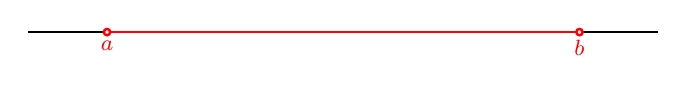
\begin{tikzpicture}
                    % \clip (0,0) rectangle (14.000000,10.000000);
                    {\footnotesize
                    
                    % Drawing line a b
                    \draw [line width=0.016cm] (1.000000,1.500000) -- (1.960000,1.500000);%
                    \draw [line width=0.016cm] (2.040000,1.500000) -- (7.960000,1.500000);%
                    \draw [line width=0.016cm] (8.040000,1.500000) -- (9.000000,1.500000);%
                    
                    % Changing color 255 0 0
                    \definecolor{r255g0b0}{rgb}{1.000000,0.000000,0.000000}%
                    \color{r255g0b0}% 
                    
                    % Drawing segment a b
                    \draw [line width=0.032cm] (2.040000,1.500000) -- (7.960000,1.500000);%
                    
                    % Marking point a by circle
                    \draw [line width=0.032cm] (2.000000,1.500000) circle (0.040000);%
                    \draw (2.000000,1.500000) node [anchor=north] { $a$ };%
                    
                    % Marking point b by circle
                    \draw [line width=0.032cm] (8.000000,1.500000) circle (0.040000);%
                    \draw (8.000000,1.500000) node [anchor=north] { $b$ };%
                    \color{black}
                    }
                    \end{tikzpicture}
                \end{figure}
                    
                
            


            \subsubsection*{Odprti interval}
            Vsebuje vsa realna števila med $a$ in $b$, vendar ne vsebuje krajišč $a$ in $b$.

                $$ \mathbf{(a,b)=\left\{x\in\mathbb{R}; a<x<b\right\} }$$


                \begin{figure}[H]
                    \centering
                    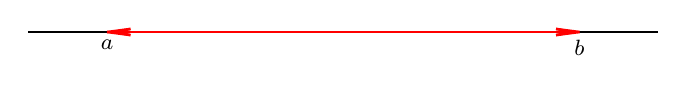
\begin{tikzpicture}
                    % \clip (0,0) rectangle (14.000000,10.000000);
                    {\footnotesize
                    
                    % Drawing line a b
                    \draw [line width=0.016cm] (1.000000,1.500000) -- (9.000000,1.500000);%
                    
                    % Changing color 255 0 0
                    \definecolor{r255g0b0}{rgb}{1.000000,0.000000,0.000000}%
                    \color{r255g0b0}% 
                    
                    % Drawing segment a b
                    \draw [line width=0.032cm] (2.000000,1.500000) -- (8.000000,1.500000);%
                    
                    % Drawing arrow a b 1.00
                    \draw [line width=0.032cm] (7.702567,1.539158) -- (8.000000,1.500000);%
                    \draw [line width=0.032cm] (7.702567,1.539158) -- (7.900856,1.500000);%
                    \draw [line width=0.032cm] (7.702567,1.460842) -- (8.000000,1.500000);%
                    \draw [line width=0.032cm] (7.702567,1.460842) -- (7.900856,1.500000);%
                    
                    % Drawing arrow b a 1.00
                    \draw [line width=0.032cm] (2.297433,1.460842) -- (2.000000,1.500000);%
                    \draw [line width=0.032cm] (2.297433,1.460842) -- (2.099144,1.500000);%
                    \draw [line width=0.032cm] (2.297433,1.539158) -- (2.000000,1.500000);%
                    \draw [line width=0.032cm] (2.297433,1.539158) -- (2.099144,1.500000);%
                    \color{black}
                        
                    % Marking point a
                    \draw (2.000000,1.500000) node [anchor=north] { $a$ };%
                    
                    % Marking point b
                    \draw (8.000000,1.500000) node [anchor=north] { $b$ };%
                    }
                    \end{tikzpicture}
                \end{figure}

                
            
            

        

        
            
            \subsubsection*{Polodprti/polzaprti interval}
                \begin{itemize}
                    \item Vsebuje vsa realna števila med $a$ in $b$, vključno s krajiščem $a$, vendar ne vsebuje krajišča $b$.
                    $$ \mathbf{[a,b)=\left\{x\in\mathbb{R}; a\leq x<b\right\} }$$


                    \begin{figure}[H]
                        \centering
                        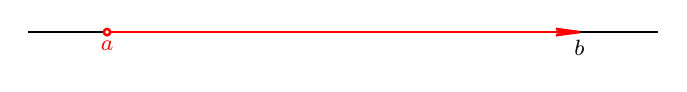
\begin{tikzpicture}
                        % \clip (0,0) rectangle (14.000000,10.000000);
                        {\footnotesize
                        
                        % Drawing line a b
                        \draw [line width=0.016cm] (1.000000,1.500000) -- (1.960000,1.500000);%
                        \draw [line width=0.016cm] (2.040000,1.500000) -- (9.000000,1.500000);%
                        
                        % Changing color 255 0 0
                        \definecolor{r255g0b0}{rgb}{1.000000,0.000000,0.000000}%
                        \color{r255g0b0}% 
                        
                        % Drawing segment a b
                        \draw [line width=0.032cm] (2.040000,1.500000) -- (8.000000,1.500000);%
                        
                        % Marking point a by circle
                        \draw [line width=0.032cm] (2.000000,1.500000) circle (0.040000);%
                        \draw (2.000000,1.500000) node [anchor=north] { $a$ };%
                        
                        % Drawing arrow a b 1.00
                        \draw [line width=0.032cm] (7.702567,1.539158) -- (8.000000,1.500000);%
                        \draw [line width=0.032cm] (7.702567,1.539158) -- (7.900856,1.500000);%
                        \draw [line width=0.032cm] (7.702567,1.460842) -- (8.000000,1.500000);%
                        \draw [line width=0.032cm] (7.702567,1.460842) -- (7.900856,1.500000);%
                        \color{black}
                        
                        % Marking point b
                        \draw (8.000000,1.500000) node [anchor=north] { $b$ };%
                        }
                        \end{tikzpicture}
                    \end{figure}

                        
                    
                    

                    \item Vsebuje vsa realna števila med $a$ in $b$, vključno s krajiščem $b$, vendar ne vsebuje krajišča $a$.
                    $$ \mathbf{(a,b]=\left\{x\in\mathbb{R}; a<x\leq b\right\} }$$


                    \begin{figure}[H]
                        \centering
                        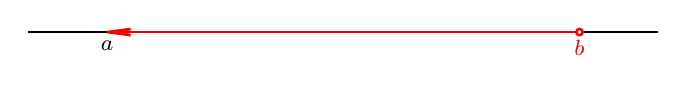
\begin{tikzpicture}
                        % \clip (0,0) rectangle (14.000000,10.000000);
                        {\footnotesize
                        
                        % Drawing line a b
                        \draw [line width=0.016cm] (1.000000,1.500000) -- (7.960000,1.500000);%
                        \draw [line width=0.016cm] (8.040000,1.500000) -- (9.000000,1.500000);%
                        
                        % Changing color 255 0 0
                        \definecolor{r255g0b0}{rgb}{1.000000,0.000000,0.000000}%
                        \color{r255g0b0}% 
                        
                        % Drawing segment a b
                        \draw [line width=0.032cm] (2.000000,1.500000) -- (7.960000,1.500000);%
                        
                        % Marking point b by circle
                        \draw [line width=0.032cm] (8.000000,1.500000) circle (0.040000);%
                        \draw (8.000000,1.500000) node [anchor=north] { $b$ };%
                        
                        % Drawing arrow b a 1.00
                        \draw [line width=0.032cm] (2.297433,1.460842) -- (2.000000,1.500000);%
                        \draw [line width=0.032cm] (2.297433,1.460842) -- (2.099144,1.500000);%
                        \draw [line width=0.032cm] (2.297433,1.539158) -- (2.000000,1.500000);%
                        \draw [line width=0.032cm] (2.297433,1.539158) -- (2.099144,1.500000);%
                        \color{black}

                        % Marking point a
                        \draw (2.000000,1.500000) node [anchor=north] { $a$ };%
                        }
                        \end{tikzpicture}
                    \end{figure}

                        
                    

                \end{itemize}


            
            
        

        
            \subsubsection*{Neomejeni/neskončni intervali}
                
                \begin{itemize}
                    \item $ \mathbf{[a,\infty)=\left\{x\in\mathbb{R}; x\geq a\right\} }$ \\

                    \begin{figure}[H]
                    \centering
                        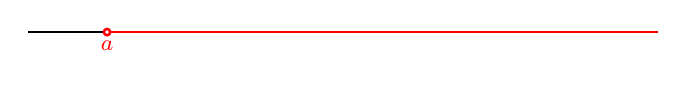
\begin{tikzpicture}
                        % \clip (0,0) rectangle (14.000000,10.000000);
                        {\footnotesize
                        
                        % Drawing line a b
                        \draw [line width=0.016cm] (1.000000,1.500000) -- (1.960000,1.500000);%
                        \draw [line width=0.016cm] (2.040000,1.500000) -- (9.000000,1.500000);%
                        
                        % Changing color 255 0 0
                        \definecolor{r255g0b0}{rgb}{1.000000,0.000000,0.000000}%
                        \color{r255g0b0}% 
                        
                        % Drawing segment a y
                        \draw [line width=0.032cm] (2.040000,1.500000) -- (9.000000,1.500000);%
                        
                        % Marking point a by circle
                        \draw [line width=0.032cm] (2.000000,1.500000) circle (0.040000);%
                        \draw (2.000000,1.500000) node [anchor=north] { $a$ };%
                        \color{black}
                        }
                        \end{tikzpicture}
                    \end{figure}
                        
                    \item $ \mathbf{(a,\infty)=\left\{x\in\mathbb{R}; x>a\right\} }$ \\
                    
                    \begin{figure}[H]
                        \centering
                        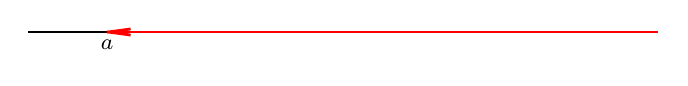
\begin{tikzpicture}
                        % \clip (0,0) rectangle (14.000000,10.000000);
                        {\footnotesize
                        
                        % Drawing line a b
                        \draw [line width=0.016cm] (1.000000,1.500000) -- (9.000000,1.500000);%
                        
                        % Marking point a
                        \draw (2.000000,1.500000) node [anchor=north] { $a$ };%
                        
                        % Changing color 255 0 0
                        \definecolor{r255g0b0}{rgb}{1.000000,0.000000,0.000000}%
                        \color{r255g0b0}% 
                        
                        % Drawing segment a y
                        \draw [line width=0.032cm] (2.000000,1.500000) -- (9.000000,1.500000);%
                        
                        % Drawing arrow b a 1.00
                        \draw [line width=0.032cm] (2.297433,1.460842) -- (2.000000,1.500000);%
                        \draw [line width=0.032cm] (2.297433,1.460842) -- (2.099144,1.500000);%
                        \draw [line width=0.032cm] (2.297433,1.539158) -- (2.000000,1.500000);%
                        \draw [line width=0.032cm] (2.297433,1.539158) -- (2.099144,1.500000);%
                        \color{black}
                        }
                        \end{tikzpicture}
                    \end{figure}

                        
                    \item $\mathbf{(-\infty,b]=\left\{x\in\mathbb{R}; x\leq b\right\} }$ \\
                    
                    \begin{figure}[H]
                        \centering
                        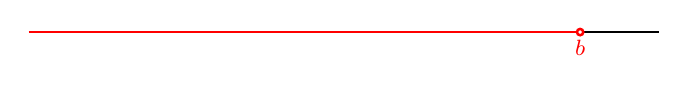
\begin{tikzpicture}
                        % \clip (0,0) rectangle (14.000000,10.000000);
                        {\footnotesize
                        
                        % Drawing line a b
                        \draw [line width=0.016cm] (1.000000,1.500000) -- (7.960000,1.500000);%
                        \draw [line width=0.016cm] (8.040000,1.500000) -- (9.000000,1.500000);%
                        
                        % Changing color 255 0 0
                        \definecolor{r255g0b0}{rgb}{1.000000,0.000000,0.000000}%
                        \color{r255g0b0}% 
                        
                        % Marking point b by circle
                        \draw [line width=0.032cm] (8.000000,1.500000) circle (0.040000);%
                        \draw (8.000000,1.500000) node [anchor=north] { $b$ };%
                        
                        % Drawing segment x b
                        \draw [line width=0.032cm] (1.000000,1.500000) -- (7.960000,1.500000);%
                        \color{black}
                        }
                        \end{tikzpicture}
                    \end{figure}

                        
                    \item $ \mathbf{(-\infty,b)=\left\{x\in\mathbb{R}; x<b\right\} }$ \\
                    
                    \begin{figure}[H]
                        \centering
                        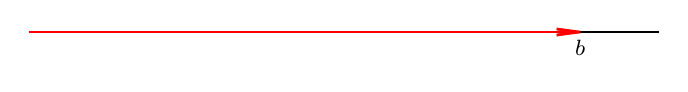
\begin{tikzpicture}
                        % \clip (0,0) rectangle (14.000000,10.000000);
                        {\footnotesize
                        
                        % Drawing line a b
                        \draw [line width=0.016cm] (1.000000,1.500000) -- (9.000000,1.500000);%
                        
                        % Marking point b
                        \draw (8.000000,1.500000) node [anchor=north] { $b$ };%
                        
                        % Changing color 255 0 0
                        \definecolor{r255g0b0}{rgb}{1.000000,0.000000,0.000000}%
                        \color{r255g0b0}% 
                        
                        % Drawing segment x b
                        \draw [line width=0.032cm] (1.000000,1.500000) -- (8.000000,1.500000);%
                        
                        % Drawing arrow a b 1.00
                        \draw [line width=0.032cm] (7.702567,1.539158) -- (8.000000,1.500000);%
                        \draw [line width=0.032cm] (7.702567,1.539158) -- (7.900856,1.500000);%
                        \draw [line width=0.032cm] (7.702567,1.460842) -- (8.000000,1.500000);%
                        \draw [line width=0.032cm] (7.702567,1.460842) -- (7.900856,1.500000);%
                        \color{black}
                        }
                        \end{tikzpicture}
                    \end{figure}

                    \item $ \mathbf{(-\infty,\infty)=\left\{x;x\in\mathbb{R}\right\} =\mathbb{R}}$ \\
                    
                    \begin{figure}[H]
                        \centering
                        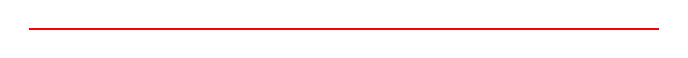
\begin{tikzpicture}
                            % \clip (0,0) rectangle (14.000000,10.000000);
                            {\footnotesize
                            
                            % Drawing line a b
                            \draw [line width=0.016cm] (1.000000,1.500000) -- (9.000000,1.500000);%
                            
                            % Changing color 255 0 0
                            \definecolor{r255g0b0}{rgb}{1.000000,0.000000,0.000000}%
                            \color{r255g0b0}% 
                            
                            % Drawing segment x y
                            \draw [line width=0.032cm] (1.000000,1.500000) -- (9.000000,1.500000);%
                            \color{black}
                            }
                        \end{tikzpicture}
                    \end{figure}

                \end{itemize}

            
            
                ~~~

                \begin{multicols}{2}
        
            \begin{naloga}
                Zapišite kot interval.
                \begin{itemize}
                        \item $\{x\in\mathbb{R}; -2<x<2\}$ 
                        \item $\{x\in\mathbb{R}; 4\leq x\leq 2\}$ 
                        \item $\{x\in\mathbb{R}; -14<x\leq -9\}$ 
                \end{itemize}
            \end{naloga}
        


        
            \begin{naloga}
                Zapišite interval, ki je narisan na sliki.
                \begin{itemize}
                        \item $ $ 
                        \item $ $ 
                        \item $ $ 
                \end{itemize}
            \end{naloga}
        


        
            \begin{naloga}
                Zapišite presek intervalov.
                \begin{itemize}
                    
                        \item $ [0,2)\cap(-1,1]$ 
                        \item $ [-3,5]\cap(-3,5)$ 
                        \item $ [2,5)\cap[5,7)$ 
                        \item $ [-1,3)\cap(-4,-1]$ 
                        \item $ [4,6]\cap[-1,4]$ 
                        \item $ (-1,3)\cap[1,2)$ 
                    

                \end{itemize}
            \end{naloga}
        


        
            \begin{naloga}
                Zapišite unijo intervalov.
                \begin{itemize}
                        \item $ [0,2)\cup(-1,1]$ 
                        \item $ [-3,5]\cup(-3,5)$ 
                        \item $ [2,5)\cup[5,7)$ 
                        \item $ [-1,3)\cup(-4,1]$ 
                \end{itemize}
            \end{naloga}
        


        
        
            \begin{naloga}
                Zapišite razliko intervalov.
                \begin{itemize}
                        \item $ [2,3]\setminus[3,4)$ 
                        \item $ (1,3)\setminus(3,4)$ 
                        \item $ [2,5)\setminus(-1,2]$ 
                        \item $ (2,8)\setminus[5,6)$ 
                \end{itemize}
            \end{naloga}
        


        
            \begin{naloga}
                Izračunajte.
                \begin{itemize}
                        \item $\left([1,3)\setminus(1,4]\right)\cup(1,2)$ 
                        \item $[-2,4]\setminus\left((-1,2]\cap[0,3)\right)$ 
                        \item $\left((-2,3]\setminus[-3,2)\right)\cap[3,5)$ 
                \end{itemize}
            \end{naloga}
        
        \end{multicols}

    
\end{priprava}
\begin{priprava}{9., 10., 11}{}{Reševanje enačb}{Realna števila}{frontalna}{drsnice, projekcija, tabla}
    
    \section{Reševanje enačb}

        
                \textbf{Enačba} je enakost dveh izrazov, pri čemer vsaj v enem nastopa \textbf{neznanka}, ki je ponavadi označena s črko $x$.

                \textbf{Rešitev enačbe} je vsaka vrednost neznanke, za katero sta vrednosti leve in desne strani enačbe enaki.
            
~

                Enačbo rešujemo tako, da jo preoblikujemo v ekvivalentno enačbo, iz katere preberemo rešitve.

                Ekvivalentno enačbo dobimo, če:
                \begin{itemize}
                    \item na obeh straneh enačbe prištejemo isto število ali izraz;
                    \item obe strani enačbe množimo z istim neničelnim številom ali izrazom.
                \end{itemize}
            
        
                ~~\\
        
                \textbf{Linearna enačba} je enačba oblike $ax+b=0;~a,b\in\mathbb{R}$.

                Rešujemo jo tako, da jo preoblikujemo v ekvivalentno enačbo, ki ima na eni strani samo neznanko.
            
~~

                \textbf{Razcepna enačba} je enačba, v kateri nastopajo potence neznanke (na primer $x^2$, $x^3$) in jo je mogoče zapisati kot produkt (linearnih) faktorjev.

                Preoblikujemo jo v ekvivalentno enačbo, ki ima vse člene na eni strani neenačaja, na drugi pa $0$. 
                Izraz (neničelna stran) razstavimo, kolikor je mogoče, in preberemo rešitve.
            
~~

                \textbf{Racionalna enačba} je enačba, v kateri nastopajo neznake (tudi) v imenovalcu, pri tem smo pozorni na obstoj ulomkov. 
                Nato enačbo preoblikujemo v ekvivalentno enačbo.
            

        ~~~\\



        %%% naloge

        
            \begin{naloga}
                Rešite enačbe.
                \begin{itemize}
                        \item $3(2a-1)-5(a-2)=9$ 
                        \item $2(y-2)+3(1-y)=7$ 
                        \item $3(3-2(t-1))=3(5-t)$ 
                        \item $-(2-x)+3(x+1)=x-5$ 
                \end{itemize}
            \end{naloga}
        


        
            \begin{naloga}
                Rešite enačbe.
                \begin{itemize}
                        \item $\dfrac{1}{5}-\dfrac{x-1}{2}=\dfrac{7}{10}$ 
                        \item $\dfrac{a-1}{3}+\dfrac{a+2}{6}=\dfrac{1}{2}$ 
                        \item $2\dfrac{2}{3}-\dfrac{3t+1}{6}=0$ 
                        \item $\left(\dfrac{2}{b+1}\right)^{-1}+\dfrac{b-1}{4}=b+3$ 
                \end{itemize}
            \end{naloga}
        



        
            \begin{naloga}
                Rešite razcepne enačbe.
                \begin{itemize}
                        \item $x^2-3x=-2$ 
                        \item $(x+2)^3-(x-1)^3=8x^2+x+2$ 
                        \item $x^4=16x^2$ 
                        \item $(x^2-4x+5)^2-(x^2+4x+1)^2-78=2x^2(x+30)-18(x+1)^3$ 
                        \item $x^3-4x^2+4=x$ 
                        \item $x^5=3x^4-2x^3$ 
                \end{itemize}
            \end{naloga}
        


        
            \begin{naloga}
                Rešite enačbe.
                \begin{itemize}
                        \item $\dfrac{x-1}{x+2}=\dfrac{x+1}{x-3}$ 
                        \item $\dfrac{1}{a-1}-\dfrac{3}{a}=\dfrac{2}{a-1}$ 
                        \item $\dfrac{x-3}{x-2}+\dfrac{x+4}{x+1}=\dfrac{2x^2}{x^2-x-2}$ 
                        \item $\dfrac{1}{3a-1}+\dfrac{1}{3a+1}=\dfrac{a-1}{9a^2-1}$ 
                \end{itemize}
            \end{naloga}
        


        
            \begin{naloga}
                Neznano število smo delili s $4$ in dobljenemu količniku prišteli $1$. 
                Dobili smo enako, kot če bi istemu številu prišteli $10$. Izračunajte neznano število.
                
            \end{naloga}

            \begin{naloga}
                Kvadrat neznanega števila je za $4$ manjši od njegovega štirikratnika. Izračunajte neznano število.
                
            \end{naloga}

        


        
            \begin{naloga}
                Avtomobil vozi s povprečno hitrostjo $50~\frac{km}{h}$, kolesar s povprečno hitrostjo $20~\frac{km}{h}$.
                Avtomobil gre iz Lendave v Ormož (približno $50~km$), kolesar vozi v obratno smer. 
                Koliko časa pred avtomobilom mora na pot kolesar, da se bosta srečala na polovici poti?
                
            \end{naloga}

            \begin{naloga}
                Vsota števk dvomestnega števila je $3$. Če zamenjamo njegovi števki, dobimo za $9$ manjše število. Katero število je to?
                
            \end{naloga}

        


        
            \begin{naloga}
                Andreja je bila ob rojstvu hčere Eve stara $38$ let. Čez koliko let bo Andreja stara trikrat toliko kot Eva?
                
            \end{naloga}

            \begin{naloga}
                Prvi delavec sam pozida steno v  $10$ urah, drugi v $12$ urah, tretji v $8$ urah. 
                Delavci skupaj začnejo zidati steno. Po dveh urah tretji delavec odide, pridruži pa se četrti delavec. 
                Skupaj s prvim in drugim delavcem nato končajo steno v eni uri. V kolikšnem času četrti delavec pozida steno?
                
            \end{naloga}

        



    
\end{priprava}
\begin{priprava}{12., 13}{}{Reševanje neenačb}{Realna števila}{frontalna}{drsnice, projekcija, tabla}
    
    \section{Reševanje neenačb}

        

                \textbf{Neenačba} je neenakost dveh izrazov, pri čemer vsaj v enem nastopa neznanka.
                Med levo in desno stranjo je postavljen eden od neenačajev: $<$, $>$, $\leq$ ali $\geq$.

                ~

                Neenačbo rešujemo tako, da jo preoblikujemo v ekvivalentno neenačbo. To dobimo, če:
                \begin{itemize}
                    \item prištejemo isto število ali izraz na obeh straneh neenačbe;
                    \item množimo obe strani neenačbe z istim pozitivnim številom ali izrazom;
                    \item množimo obe strani neenačbe z istim negativnim številom ali izrazom in se pri tem neenačaj obrne.
                \end{itemize}
            
                ~
            
                \textbf{Linearna neenačba} je oblike $ax+b<0$, ali pa nastopa drug neenačaj: $>$, $\leq$, $\geq$.
            
        
~~~\\



                %%% naloge
        
                
                    \begin{naloga}
                        Poiščite vsa realna števila, ki ustrezajo pogoju.
                        \begin{itemize}
                                \item $3a+2<2a-1$ 
                                \item $7t+8\geq 8(t-2)$ 
                                \item $5x-2>2(x+1)-3$ 
                                \item $x-1\leq 2(x-3)-x$ 
                        \end{itemize}
                    \end{naloga}
                
        
        
                
                    \begin{naloga}
                        Rešite neenačbe.
                        \begin{itemize}
                                \item $\dfrac{x}{2}+\dfrac{2}{3}<\dfrac{8}{3}$ 
                                \item $\dfrac{4+5a}{34}-\dfrac{4}{51}\geq 2+\dfrac{2-a}{51}$ 
                                \item $x+\dfrac{x-2}{3}<\dfrac{x-3}{4}+\dfrac{x-1}{2}$ 
                                \item $\dfrac{2x-2}{15}+\dfrac{x}{3}<\dfrac{4x-2}{5}+\dfrac{3x+9}{10}$ 
                        \end{itemize}
                    \end{naloga}
                
        
        
        
                
                    \begin{naloga}
                        Rešite sisteme neenačb.
                        \begin{itemize}
                                \item $-2<y-2<1$ 
                                \item $-4\leq 5a-9\leq 1$ 
                                \item $(x+1>3)\land (2x\leq 3(x-1))$ 
                                \item $(3x-5<x+3)\lor (2x\geq x+6)$ 
                        \end{itemize}
                    \end{naloga}
                
        

    
\end{priprava}
\begin{priprava}{14., 15., 16}{}{Reševanje sistemov enačb}{Realna števila}{frontalna}{drsnice, projekcija, tabla}
    
    \section{Reševanje sistemov enačb}

        

            \subsection{Sistem dveh linearnih enačb z dvema neznankama}

                \textbf{Sistem dveh linearnih enačb z dvema neznankama} ali \textbf{sistem $\mathbf{2\times 2}$} je v splošnem oblike:
                    $$\begin{aligned}
                            a_1x+b_1y&=c_1 \\ a_2x+b_2y&=c_2
                        \end{aligned}$$
                $x$ in $y$ sta \textbf{neznanki}, $a_i,b_i,c_i\in\mathbb{R}$ so \textbf{koeficienti}.
            
~
            
                \textbf{Rešitev sistema} je \textbf{urejen par} števil $(x,y)$, ki zadoščajo obema enačbama.
            

            
                    Sistem $2\times 2$ ima lahko eno rešitev, nima rešitve ali ima neskončno rešitev.
            

        

        
            
                Sistem lahko rešujemo s primerjalnim načinom, zamenjalnim načinom ali z metodo nasprotnih koeficientov.
            
        
            \subsubsection*{Primerjalni način}
                Iz obeh enačb izrazimo isto neznanko, nato njuni vrednosti enačimo.
            

            \subsubsection*{Zamenjalni način}
                Iz ene enačbe izrazimo eno izmed neznank (preverimo, če je kateri od koeficientov pri neznankah enak $1$ -- takšno neznanko hitro izrazimo) in izraženo vrednost vstavimo v drugo enačbo.
            

            \subsubsection*{Metoda nasprotnih koeficientov}
                Eno ali obe enačbi pomnožimo s takimi števili, da bosta pri eni izmed neznank koeficienta nasprotni števili, nato enačbi seštejemo.
                Ostane ena enačba z eno neznanko.
            

~~~\\
        

        %%% naloge

        
            \begin{naloga}
                Rešite sisteme enačb.
                \begin{itemize}
                    
                        \item $\begin{aligned}
                            2x+y&=9 \\ x-3y&=8
                        \end{aligned}$ 
                        \item $\begin{aligned}
                            x-y&=5 \\ y-x&=3
                        \end{aligned}$ 
                        \item $\begin{aligned}
                            2x-3y&=5 \\ -4x+6y&=-10
                        \end{aligned}$ 
                        \item $\begin{aligned}
                            3x-y&=5 \\ 6x-10&=2y
                        \end{aligned}$ 
                    

                \end{itemize}
            \end{naloga}
        


        
            \begin{naloga}
                Z zamenjalnim načinom rešite sisteme enačb.
                \begin{itemize}
                    
                        \item $\begin{aligned}
                            2x+5y&=-2 \\ x-3y&=-1
                        \end{aligned}$ 
                        \item $\begin{aligned}
                            \frac{x}{2}-y&=3 \\ y+x&=-2
                        \end{aligned}$ 
                        \item $\begin{aligned}
                            3x-2y&=1 \\ x+y&=\frac{7}{6}
                        \end{aligned}$ 
                        \item $\begin{aligned}
                            0.5x+0.2y&=2 \\ \frac{3}{2}x-\frac{2}{5}y&=1
                        \end{aligned}$ 
                    

                \end{itemize}
            \end{naloga}
        


        
            \begin{naloga}
                Z metodo nasprotnih koeficientov rešite sisteme enačb.
                \begin{itemize}
                    
                        \item $\begin{aligned}
                            2x+3y&=3 \\ -4x+3y&=0
                        \end{aligned}$ 
                        \item $\begin{aligned}
                            4x-3y&=-2 \\ -8x+y&=-1
                        \end{aligned}$ 
                        \item $\begin{aligned}
                            3x-2y&=2 \\ 2x-3y&=-2
                        \end{aligned}$ 
                        \item $\begin{aligned}
                            x-y&=-5 \\ 0.6x+0.4y&=7
                        \end{aligned}$ 
                    

                \end{itemize}
            \end{naloga}
        


        
            \begin{naloga}
                V bloku je $26$ stanovanj. Vsako stanovanje ima $2$ ali $3$ sobe. Koliko je posameznih vrst stanovanj, če je v bloku $61$ sob?
                
            \end{naloga}

            \begin{naloga}
                Kmet ima v ogradi $20$  živali. Če so v ogradi le race in koze, koliko je posameznih živali, če smo našteli $50$ nog? 
                
            \end{naloga}

        


        
            \begin{naloga}
                Razredničarka na sladoled pelje svojih $30$ dijakov. Naročili so lahko $2$ ali $3$ kepice sladoleda. Koliko dijakov je naročilo dve in koliko tri kepice sladoleda,
                če razredničarka ni jedla sladoleda, plačala pa je $79$ kepic sladoleda?
                
            \end{naloga}

            \begin{naloga}
                Babica ima dvakrat toliko vnukinj kot vnukov. Vnukinjam je podarila po tri bombone, vnukom pa po štiri bombone.
                Koliko vnukinj in vnukov ima, če je podarila $70$ bombonov?
                
            \end{naloga}

        


~~~\\
      
            
            \subsection{Sistem treh linearnih enačb s tremi neznankami}

                \textbf{Sistem treh linearnih enačb z tremi neznankami} ali \textbf{sistem $\mathbf{3\times 3}$} je v splošnem oblike:
                    $$\begin{aligned}
                            a_1x+b_1y+c_1z&=d_1 \\ a_2x+b_2y+c_2z&=d_2 \\ a_3x+b_3y+c_3z&=d_3
                        \end{aligned}$$
                $x$, $y$ in $z$ so \textbf{neznanke}, $a_i,b_i,c_i\in\mathbb{R}$ so \textbf{koeficienti}.
            
~
            
                \textbf{Rešitev sistema} je \textbf{urejena trojka} števil $(x,y,z)$, ki zadoščajo vsem trem enačbam.
            

            
                    Sistem $3\times 3$ rečujemo z istimi postopki kot sisteme $2\times 2$, le da postopek ponovimo večkrat.
            

        
~~~\\


        
            \begin{naloga}
                Z metodo nasprotnih koeficientov rešite sisteme enačb.
                \begin{itemize}
                    
                        \item $\begin{aligned}
                            2x+y-3z&=5 \\ x+2y+2z&=1 \\ -x+y+z&=-4
                        \end{aligned}$ 
                        \item $\begin{aligned}
                            x-2y+6z&=5 \\ -x+3z&=-1 \\ 4y-3z&=-3
                        \end{aligned}$ 
                        \item $\begin{aligned}
                            x+y-z&=0 \\ x-y-3z&=2 \\ 2x+y-3z&=1
                        \end{aligned}$ 
                        \item $\begin{aligned}
                            2x-4y+z&=3 \\ 4x-y+2z&=4 \\ -8x+2y-4z&=7
                        \end{aligned}$ 
                    

                \end{itemize}
            \end{naloga}
        

    
\end{priprava}
\begin{priprava}{17}{}{Obravnava enačb in neenačb}{Realna števila}{frontalna}{drsnice, projekcija, tabla}
    
    \section{Obravnava enačb in neenačb}

        

            
            Kadar v enačbi oziroma neenačbi poleg neznake $x$ nastopajo tudi druge črke, na primer $a, b, c, k, l ...$, 
            le-te označujejo števila, ki imajo poljubno realno vrednost. Imenujemo jih \textbf{parametri}.

~
            
            Vrednost parametrov vpliva na rešitev enačbe oziroma neenačbe, zato moramo enačbo reševati glede na vrednosti parametrov.
            Temu postopku rečemo \textbf{obravnava enačbe} oziroma \textbf{obravnava neenačbe}.

        

~~~
        %%%% naloge

        
            \begin{naloga}
                Obravnavajte enačbe.
                \begin{itemize}
                        \item $2(ax-3)+3=ax$ 
                        \item $-4x-b(x-2)^2=3-bx^2-7b$ 
                        \item $3(a-2)(x-2)=a^2(x-1)-4x+7$ 
                        \item $(b-3)^2x-3=4x-3b$ 
                \end{itemize}
            \end{naloga}
        

        
            \begin{naloga}
                Obravnavajte neenačbe.
                \begin{itemize}
                        \item $a(x-2)\leq 4$ 
                        \item $mx+4>m^2-2x$ 
                        \item $a(a-3x+1)\geq a(x-4)+a^2x$ 
                        \item $(k-1)^2x\leq kx+2(k+1)+5x$ 
                \end{itemize}
            \end{naloga}

    
\end{priprava}
\begin{priprava}{18}{}{Sklepni račun}{Realna števila}{frontalna}{drsnice, projekcija, tabla}
    
    \section{Sklepni račun}

    

        
            Pri sklepnem računu obravnavamo situacije, v katerih nastopata dve količini,
            ki sta premo sorazmerni ali obratno sorazmerni.
        

        \subsubsection*{Premo sorazmerje}
        Količini $x$ in $y$ sta \textbf{premo sorazmerni}, če obstaja takšno neničelno število $k\in\mathbb{R}^*$, da je $x=k\cdot y$.
        

        \subsubsection*{Obratno sorazmerje}
        Količini $x$ in $y$ sta \textbf{obratno sorazmerni}, če obstaja takšno neničelno število $k\in\mathbb{R}^*$, da je $x=\dfrac{k}{y}$.
        

    
~~~~\\

    %%% naloge

    
        \begin{naloga}
            Delavec v štirih urah zasluži $10~€$. Koliko zasluži v dvanajstih urah?            
        \end{naloga}

        \begin{naloga}
            Tiskalnik v sedmih minutah natisne $42$ strani. Koliko časa potrebuje za $108$ strani?            
        \end{naloga}

        \begin{naloga}
            Tri čebele v treh dneh oprašijo devetsto cvetov. Koliko cvetov v šestih dneh opraši šest čebel?            
        \end{naloga}
 
        \begin{naloga}
            Kolesar od Ljubljane do Geometrijskega središča Slovenije potuje dve uri s hitrostjo $20~km/h$. 
            Kako hitro bi moral peljati, da bi pot prevozil v eni uri in petnajstih minutah?            
        \end{naloga}
        
        \begin{naloga}
            En računalnik za pripravo posebnih efektov filma potrebuje $14$ ur.
            Koliko časa bi potrebovali trije taki računalniki, za pripravo posebnih efektov za šest filmov?            
        \end{naloga}

        \begin{naloga}
            Sedem pleskarjev pleska hišo $15$ dni. Po petih dneh dva delavca premestijo na drugo delovišče.
            Koliko časa bodo preostali delavci pleskali hišo?            
        \end{naloga}

    

    
\end{priprava}
\begin{priprava}{19., 20., 21}{}{Odstotni račun}{Realna števila}{frontalna}{drsnice, projekcija, tabla}
    
    \section{Odstotni račun}  
        
    Količine pri odstotnem računu so povezane s sklepnim računim, in sicer so v premem sorazmerju.

~\\
    \textbf{Odstotek} (ali procent) $\text{\%}$ celote definiramo kot stotino celote,
    \textbf{odtisoček} (ali promil) $\permil$ kot tisočino celote.

    $$ 1~\text{\%}=\dfrac{1}{100} \quad \quad {1~\permil=\dfrac{1}{1000}}$$



    \textbf{Relativni delež} je kvocient med deležem in osnovo: $r=\dfrac{d}{o}$.



~~~\\
%%%%%%% naloge

\begin{multicols}{2}
\begin{naloga}
    Zapišite z okrajšanim ulomkom oziroma odstotkom.
    \begin{multicols}{2}
    \begin{itemize}
            \item $12~\%$ 
            \item $20~\%~a$ 
            \item $250~\%$ 
            \item $0.5~\%~b$ 
            \item $12~\permil$ 
            \item $\frac{3}{4}a$ 
            \item $\frac{7}{20}x$ 
            \item $\frac{31}{10}y$ 
            \item $0.8 z$ 
            \item $\frac{25}{8}m$
    \end{itemize} 
\end{multicols}
\end{naloga}




\begin{naloga}
    Izračunajte.
    \begin{itemize}
            \item Koliko je $20~\%$ od $10~kg$? 
            \item Koliko je $25~\%$ od $20~€$? 
            \item Koliko je $10~\%$ od $1~l$? 
            \item Koliko je $250~\%$ od $12~g$? 
            \item Koliko je $1~\permil$ od $2350~kg$? 
            \item Koliko je $17~\permil$ od $100~m$? 
    \end{itemize} ~
\end{naloga}

\end{multicols}
    
    
        \begin{naloga}
            Pri ekološki pridelavi kmet pridela $3$ tone pšenice na hektar. 
            Zaradi toče je bil letošnji pridelek le $2450~kg$ pšenice.
            Za koliko odstotkov se je zmanjšala količina pridelka zaradi toče? 
        \end{naloga}

        \begin{naloga}
            V $5~kg$ raztopine je $120~g$ soli. Koliko odstotna je ta raztopina? 
        \end{naloga}

        \begin{naloga}
            V tovarni čevljev so povečali proizvodnjo s $1250$ parov tedensko na $1700$ parov.
            Koliko odstotno je to povečanje? 
        \end{naloga}
    

    
        \begin{naloga}
            Kokoši nesnice znesejo $270$ jajc letno. 
            Koliko odstotna je njihova nesnost? 
        \end{naloga}

        \begin{naloga}
            V trgovini stane izdelek $120~€$. Koliko stane po:
            \begin{itemize}
                \item $5~\%$ podražitvi,
                \item $20~\%$ pocenitvi?
            \end{itemize}
        \end{naloga}

        \begin{naloga}
            Jošt je natipkal besedilo na list A4 formata v pisava Arial, velikosti $12$, in ugotovil, da je bilo na strani $3150$ znakov s presledki.
            Če bi pisavo zmanjšal na velikost $10$, bi na stran prišlo $28~\%$ več znakov. Koliko? 
        \end{naloga}
    

    
    
        \begin{naloga}
            Dizelsko gorivo je stalo v Sloveniji $1.421~€$, v Italijo $1.748~€$, v Avstriji pa $1.751~€$.
            Za koliko odstotkov je bilo gorivo v Italiji dražje od goriva v naši državi in za koliko odstotkov je bilo
            naše gorivo cenejše od goriva v Avstriji? 
        \end{naloga}

        \begin{naloga}
            Prenočitvene zmogljivosti na Bledu so $8880$ ležišč. Pred prvomajskimi prazniki so se turistični delavci pohvalili,
            da je zasedenost kapacitet $90~\%$. Koliko turistov še lahko sprejmejo na nočitev? 
        \end{naloga}

        \begin{naloga}
            Maksov avto porabi $5.6~l$ goriva na prevoženih $100~km$. 
            Z varčno vožnjo lahko zniža porabo za $15~\%$.
            Koliko kilometrov bo tako prevozil s polnim rezervoarjem, ki drži $55~l$. 
        \end{naloga}
    


    
        \begin{naloga}
            Kavču, ki je stal $652~€$, so ceno znižali za $10~\%$, na sejmu pa so ponudili na to ceno še $12~\%$ sejemskega popusta.
            Koliko bomo odšteli za kavč na sejmu? Za koliko odstotkov je cena na sejmu nižja od prvotne cene kavča? 
        \end{naloga}

        
        \begin{naloga}
            Servis so najprej podražili za $10~\%$, potem pa se je ena skodelica okrušila in so ga pocenili za $30~\%$.
            Koliko je servis stal na začetku, če ga danes lahko kupimo za $115.5~€$? 
        \end{naloga}

        \begin{naloga}
            Izdelek je imel napako, zato so ga pocenili za $20~\%$. Ko so napako skoraj v celoti odpravili, so ga podražili za $20~\%$.
            Kolikšna je bila začetna cena izdelka, če po popravilu stane $192~€$? 
        \end{naloga}

    


    
        \begin{naloga}
            Koliko vode moramo priliti $3~kg$ $45~\%$ raztopine, da bomo koncentracijo znižali na $20~\%$? 
        \end{naloga}

        \begin{naloga}
            Kolikšno koncentracijo raztopine dobimo, če zmešamo $2~kg$ $60~\%$ raztopine in $3~kg$ $40~\%$ raztopine? 
        \end{naloga}

        \begin{naloga}
            Koliko $kg$ $12~\%$ raztopine moramo priliti k $30~kg$ $24~\%$ raztopine, da bomo dobili raztopino z $20~\%$ koncentracijo? 
        \end{naloga}
    


    
\end{priprava}
\begin{priprava}{22., 23., 24., 25}{}{Absolutna vrednost}{Realna števila}{frontalna}{drsnice, projekcija, tabla}
    
    \section{Absolutna vrednost}

        
    \textbf{Absolutna vrednost} $|x|$ števila $x$ geometrijsko predstavlja oddaljenost točke, 
    ki predstavlja število $x$, od izhodišča na številski premici.



    $$|x|=\begin{cases} x &x\geq 0; \\ -x & x<0. \end{cases}$$


\subsubsection*{Lastnosti absolutne vrednosti}
            \begin{itemize}
                \item $|x|\geq 0$
                \item $|x|=0 \Leftrightarrow x=0$
                \item $|-x|=|x|$
                \item $|x\cdot y|=|x|\cdot|y|$
                \item $|x+y|\leq |x|+|y|$ -- \textbf{trikotniška neenakost}
            \end{itemize}

~


    Z absolutno vrednostjo izračunamo tudi razdaljo med $x$ in $y$ kot $|x-y|$ ali $|y-x|$.

~~~\\


%%%% naloge

\begin{multicols}{2}


\begin{naloga}
    Izračunajte.
    \begin{itemize}
        \item $|13|$ 
        \item $|-5|$ 
        \item $|-2|\cdot|4|$ 
        \item $|-3|-|5|$ 
        \item $|-1|\cdot|-6|$ 
        \item $-|3|+|-9|$ 
            
    \end{itemize}
\end{naloga}


\begin{naloga}
    Izračunajte.
    \begin{itemize}
        \item $\left\lvert\frac{1}{5}-5\right\rvert$ 
        \item $\left\lvert-\frac{3}{4}-\frac{2}{3}\right\rvert$ 
        \item $\left\lvert\sqrt{5}-3\right\rvert$ 
        \item $\left\lvert-1+\sqrt{2}\right\rvert$ 
        \item $\left\lvert 1-\lvert\sqrt{6}-3\rvert\right\rvert$ 
        \item $\left\lvert\lvert\sqrt{2}-2\rvert-\lvert 1-\sqrt{2}\rvert\right\rvert$ 
            
    \end{itemize}
\end{naloga}



\begin{naloga}
    Odpravite absolutno vrednost.
    \begin{itemize}

        \item $\left\lvert a-2\right\rvert$ 
        \item $\left\lvert x+1\right\rvert$ 
        \item $\left\lvert 4-b\right\rvert$ 
        \item $\left\lvert 2+e\right\rvert$ 
        \item $-\left\lvert 1-y\right\rvert$ 
        \item $-\left\lvert 3+6y\right\rvert$ 
            
    \end{itemize}
\end{naloga}

~\\

\begin{naloga}
    Poenostavite izraze.
    \begin{itemize}
            \item $x-2+\left\lvert x\right\rvert$ 
            \item $3\cdot\left\lvert x-2\right\rvert +x-1$ 
            \item $\left\lvert a-2\right\rvert+\left\lvert a\right\rvert$ 
            \item $3\cdot \left\lvert b-2\right\rvert+\left\lvert b-1 \right\rvert$ 
            \item $\left\lvert \lvert x-2\rvert +x \right\rvert$ 
            \item $3\cdot \left\lvert \lvert y-2\rvert +\lvert y-1\rvert \right\rvert$ 

    \end{itemize}
\end{naloga}


\begin{naloga}
    Rešite enačbe.
    \begin{itemize}
            \item $\left\lvert x-2 \right\rvert =3$ 
            \item $\left\lvert 3-x\right\rvert =5$ 
            \item $1+ \left\lvert x-7 \right\rvert =-6$ 
            \item $\left\lvert a+3 \right\rvert = 7- \left\lvert a+2 \right\rvert$ 
            \item $\left\lvert b-1 \right\rvert = 2 + \left\lvert b+3 \right\rvert$ 
            \item $\left\lvert x-1 \right\rvert + \left\lvert x+2 \right\rvert =3$ 

    \end{itemize}
\end{naloga}


\begin{naloga}
    Rešite neenačbe.
    \begin{itemize}
            \item $\left\lvert x-2 \right\rvert \geq 3$ 
            \item $\left\lvert 3-x\right\rvert <5$ 
            \item $1+ \left\lvert x-7 \right\rvert \leq-6$ 
            \item $\left\lvert a+3 \right\rvert < 7- \left\lvert a+2 \right\rvert$ 
            \item $\left\lvert b-1 \right\rvert \geq 2 + \left\lvert b+3 \right\rvert$ 
            \item $\left\lvert \lvert x-3\rvert +2\right\rvert <1$ 
            \item $\left\lvert x- \lvert x-3\rvert \right\rvert \geq 1$ 
            \item $\left\lvert x- \lvert 2x-1\rvert \right\rvert \geq 2$ 

    \end{itemize}
\end{naloga}

\end{multicols}

\end{priprava}
\begin{priprava}{26}{}{Zaokroževanje, približki, napake}{Realna števila}{frontalna}{drsnice, projekcija, tabla}
    
    \section{Zaokroževanje, približki, napake}

    
    \subsubsection*{Pravila zaokroževanja}
        \begin{itemize}
            \item Zadnjo števko pustimo enako, če je prva izbrisana števka manjša od $5$;
            \item zadnjo števko povečamo za $1$, če je prva izbrisana števka $5$ ali več.
        \end{itemize}
    

        ~~

    
        Zaokroževanje na \textbf{$n$ decimalnih mest} pomeni: 
        opustiti vse decimalke od $n$-tega mesta dalje in zaokrožiti.
        Primer: $\sqrt{2}\doteq 1.41$ (na $2$ decimalni mesti).
    
        ~~
    
        Zaokroževanje na \textbf{$n$ mest} pomeni, 
        da ima število v svojem zapisu $n$ števk, 
        pri pogoju, da ne štejemo ničel na začetku in na koncu.
        Primer: $\sqrt{2}\doteq 1.41$ (na $3$ mesta).
    
        ~
    
        Pri zapisu uporabimo $\doteq$, kar označuje, da smo rezultat zapisali približno in ne natančno.
    




    \subsubsection*{Absolutna in relativna napaka}
        Naj bo $x$ točna vrednost in $X$ njen \textbf{približek}.

        \textbf{Absolutna napaka} približka je $\left\lvert X-x\right\rvert$; 
        \textbf{relativna napaka} je $\dfrac{\left\lvert X-x\right\rvert}{x}$.
    
        ~~
    
        Absolutno napako zapišemo tudi $X=x\pm\epsilon$, kar pomeni, da se absolutna napaka približka $X$ razlikuje od točne vrednosti $x$ kvečjemu za $\epsilon$.
    

~~\\

%%%%%% naloge


    \begin{naloga}
        Na kartonski škatli je oznaka velikosti $50 \pm 3 ~cm$.
        Koliko je največja in koliko najmanjša velikost škatle, ki ustreza tej oznaki? 
        Ali je lahko relativna napaka velikosti $8~\%$?            
    \end{naloga}
    
    \begin{naloga}
        Pri $200~m$ vrvi smemo narediti $7~\%$ napako.
        Ali je lahko takšna vrv dolga $230~m$?
        Kako dolgi bosta najkrajša in najdaljša vrv, ki še ustrezata?            
    \end{naloga}
    
    \begin{naloga}
        V EU morajo biti banane za prodajo dolge najmanj $14~cm$. 
        V trgovino dobijo novo pošiljko banan, ki jih izmerijo, da so dolžine $13.7~cm$. 
        Njihov meter ima $5~\%$ odstopanje. 
        Ali lahko prodajajo takšne banane?            
    \end{naloga}



\end{priprava}


%% 7 Pravokotni koordinatni sistem


%% 8 Funkcija


%% 9 Premica


%% 10 Osnove statistike
\begin{priprava}{0}{}{}{Osnove statistike}{}{}

    \chapter{Osnove statistike}

    \Large{Pregled vsebine poglavja in predvidenega števila ur:}

    \begin{table}[H]
        \centering
        \begin{tabular}{||c|c||} 
        \hhline{|t:==:t|}
        \rowcolor[rgb]{0.843,0.718,0.718} 
        Tema  & Predvideno število ur   \\ 
        \hhline{|:==:|}
        Osnovni pojmi statistike & $1$    \\ 
        \hline
        Urejanje in grupiranje podatkov & $2$    \\ 
        \hline
        Mere osredinjenosti & $2$    \\ 
        \hline
        Mere razpršenosti & $2$     \\
        \hline
        Grafično prikazovanje podatkov & $2$     \\
        \hhline{|:==:|}
        Skupaj & $9$     \\
        \hhline{|b:==:b|}
        \end{tabular}
    \end{table}


\end{priprava}
\begin{priprava}{1}{}{Osnovni pojmi statistike}{Osnove statistike}{frontalna}{drsnice, projekcija}

    \section{Osnovni pojmi statistike}

        

            
                \textbf{Populacija} je množica, ki jo statistično proučujemo. 
                Element populacije imenujemo \textbf{statistična enota}. 
            
                ~
            
                \textbf{Vzorec} je podmnožica populacije, katere elementi predstavljajo največjo možno mero značilnosti celotne množice. 
                Vzorec izberemo, kadar je celotna populacija prevelika množica, da bi analizirali vse njene elemente. 
                
                \begin{itemize}
                    \item \textbf{Reprezentativen vzorec} je vzorec, ki je izbran tako, da predstavlja značilnosti celotne populacije.
                    \item \textbf{Slučajni vzorec} je vzorec, ki je izbran naključno -- vsi elementi populacije imajo enako možnost, da bodo izbrani.
                \end{itemize}

                \textbf{Numerus} je število elementov vzorca. Oznaka $N$. 
            
                ~
            
                \textbf{Statistična spremenljivka/podatek/znak} je vrednost ali lastnost, ki jo proučujemo.
            

                Vrste statističnih spremenljivk:
                \begin{itemize}
                    \item \textbf{opisne/kvalitativne} statistične spremenljivke
                    \item \textbf{vrstne/ordinalne} statistične spremenljivke
                    \item \textbf{številske/kvantitivne} statistične spremenljivke
                \end{itemize}
                
            

                Številske statistične spremenljivke:
                \begin{itemize}
                    \item \textbf{diskretne} številske spremenljivke -- zavzamejo lahko posamezne vrednosti
                    \item \textbf{zvezne} številske spremenljivke -- zavzamejo lahko vsako vrednost z nekega intervala
                \end{itemize}

            


                ~\\~\\


        %%%% naloge

        
            \begin{naloga}
                Zapišite, kaj je v danem primeru populacija, vzorec, statistična enota, spremenljivka in 
                ugotovite ali je spremenljivka opisna ali numerična in, če je numerična, ugotovite, ali je zvezna ali diskretna.
                \begin{itemize}
                        \item Na spletni strani je anketa z vprašanjem ``Ali imate doma pomivalni stroj?''. Nanjo je odgovorilo $254$ ljudi. 
                        \item V televizijski oddaji gledalci glasujejo za dva kandidata. 
                        \item Razrednik svojih $28$ dijakov vpraša, kolikšna je oddaljenost njihovega doma do šole.
                        \item Maturant piše seminarsko nalogo z naslovom ``Uporaba TikTok-a med srednješolci''. Pridobil je odgovore $369$ srednješolcev, ki so odgovarjali na vprašanje ``Ali~uporabljaš~TikTok?'' 
                        \item Znanstveniki pri raziskavi spremljajo, koliko jajc znesejo kokoši na slovenskih farmah na mesec.
                \end{itemize}
            \end{naloga}
        

        



            \begin{naloga}
                    Slovenija ima več kot $6000$ naselij. Statistični urad Republike Slovenije je januarja 2024 naredil analizo naselij glede na število prebivalcev. 
                    Rezultati so prikazani v tabeli. 

                    \begin{table}[H]
                        \centering
                        \begin{tabular}{||c|c||} 
                        \hhline{|t:==:t|}
                        \rowcolor[rgb]{0.843,0.718,0.718} 
                        velikostni razred naselja  & število naselij   \\ 
                        \hhline{|:==:|}
                        $0$ & $57$    \\ 
                        \hline
                        $1-24$ & $719$    \\ 
                        \hline
                        $25-49$ & $851$    \\ 
                        \hline
                        $50-99$ & $1256$     \\
                        \hline
                        $100-199$ & $1444$     \\
                        \hline
                        $200-499$ & $1109$     \\
                        \hline
                        $500-999$ & $359$     \\
                        \hline
                        $1000-4999$ & $199$     \\
                        \hline
                        $5000-9999$ & $23$     \\
                        \hline
                        $10000-49999$ & $16$     \\                    
                        \hline
                        $50000+$ & $2$     \\
                        \hhline{|b:==:b|}
                        \end{tabular}
                    \end{table}
                
                    Zapišite, kaj je v danem primeru populacija, statistična enota, spremenljivka in ugotovite ali je spremenljivka opisna ali numerična in, 
                    če je numerična, ugotovite ali je zvezna ali diskretna.
            \end{naloga}



\end{priprava}
\begin{priprava}{2., 3}{}{Urejanje in grupiranje podatkov}{Osnove statistike}{frontalna, delo v dvojicah/individualno}{drsnice, projekcija, računalniki}

    \section{Urejanje in grupiranje podatkov}

        

            
                Podatke, pridobljene v posamezni raziskavi, moramo najprej urediti. \\
                Če podatkov ni veliko, jih uredimo po velikosti v \textbf{ranžirno vrsto}, sicer jih združujemo v skupine, \textbf{frekvenčne razrede}.
            

            
                Podatek z največjo vrednostjo označimo z $x_{max}$, podatek z najnižjo vrednostjo pa $x_{min}$.
            
                ~
            
                \textbf{Frekvenca} $f$ statističnega znaka je posamezno število diskretnih statističnih enot iste vrednosti.
            
                ~
            
                \textbf{Frekvenčni razred} je skupina podatkov iz vzorca. Frekvenčni razredi so navadno enako široki,
                in skupaj zajamejo celoten razpon podatkov. Za zvezen nabor podatkov za frekvenčne razrede izberemo intervale (navadno oblike $[a,b)$).
            

        

        
            
                \textbf{Širina frekvenčnega razreda} $d_k$ je razlika med zgornjo ($z_k$) in spodnjo ($s_k$) mejo frekvenčnega razreda:
                $$d_k=z_k-s_k.$$
            

            
                Če so razredi enako široki, določimo njihovo širino kot kvocient med celotnim razponom podatkov $x_{max}-x_{min}$ in številom razredov.
            

            
                \textbf{Sredina frekvenčnega razred} $x_k$ je aritmetična sredina zogrnje in spodnje meje razreda: 
                $$x_k=\dfrac{z_k+s_k}{2}.$$
            
        

        
            
                Grupirane podatke predstavimo s \textbf{frekvenčno preglednico/porazdelitvijo}.
            

            
                Za podatke v frekvenčnih preglednicah računamo:
                \begin{itemize}
                    \item \textbf{(absolutno) frekvenco} $f_k$ -- število podatkov z vrednostmi v danem frekvenčnem razredu;
                    \item \textbf{relativno frekvenco} $f_k'$ -- delež celote, ki ga predstavlja število podatkov v danem frekvenčnem razredu;
                    \item \textbf{(absolutno) kumulativno frekvenco} $F_k$ -- število podatkov, katerih vrednosti zavzemajo manjšo vrednost od zgornje meje danega frekvenčnega razreda;
                    \item \textbf{relativno kumulativno frekvenco} $F_k'$ -- delež celote, ki ga predstavlja število podatkov v danem in vseh manjših frekvenčnih razredih.
                \end{itemize}
            
        
                ~\\~


                %%%% naloge
        
        
                    \begin{naloga}
                        Na šoli analizirajo količino prevzetih obrokov v jedilnici. Rezultati so zbrani v tabeli. 
        
                            \begin{table}[H]
                                \centering
                                \begin{tabular}{||c|c||} 
                                \hhline{|t:==:t|}
                                \rowcolor[rgb]{0.843,0.718,0.718} 
                                Oddelek  & Število prevzetih obrokov   \\ 
                                \hhline{|:==:|}
                                1.a & $12$    \\ 
                                \hline
                                1.b & $14$    \\ 
                                \hline
                                1.c & $20$    \\ 
                                \hline
                                2.a & $17$     \\
                                \hline
                                2.b & $16$     \\
                                \hline
                                2.c & $9$     \\
                                \hline
                                3.a & $13$     \\
                                \hline
                                3.b & $16$     \\
                                \hline
                                3.c & $14$     \\
                                \hline
                                4.a & $21$     \\                    
                                \hline
                                4.b  & $8$     \\
                                \hline
                                4.c  & $12$     \\
                                \hhline{|b:==:b|}
                                \end{tabular}
                            \end{table}
                        
                        Analizirajte podatke s frekvenčno preglednico.
                        Podatke razdelite v razrede $5-9$, $10-14$, $15-19$, $20$ in več.
                    \end{naloga}

                

                
                
                    \begin{naloga}
                        Dijaki 3.~a oddelka so zapisovali svoje pribljubljene barve. \\
                        Zapisali so jih: modra, rdeča, rdeča, zelena, rumena, rdeča, modra, zelena, modra, modra, rumena, rdeča, zelena, modra, rumena, rumena, zelena, rdeča. \\
                        Analizirajte rezultate s frekvenčno preglednico. 
                    \end{naloga}

                    \begin{naloga}
                        Lokostrelec si beleži rezultate treningov. \\
                        Vrednosti so bile: $10.3$, $10.4$, $9.9$, $9.7$, $10.2$, $8.9$, $9.4$, $10.1$, $9.0$, $10.3$, $9.5$, $10.6$. \\
                        Analizirajte rezultate s frekvenčno preglednico. 
                    \end{naloga}
                

                
        
                   \begin{naloga}
                    
                    V frekvenčni preglednici so zbrani podatki o številu sorojencev dijakov 2.~b oddelka.
                    Dopolnite preglednico.
    
                        \begin{table}[H]
                            \centering
                            \begin{tabular}{||c|c|c|c|c||} 
                            \hhline{|t:=====:t|}
                            \rowcolor[rgb]{0.843,0.718,0.718} 
                            Število sorojencev  & $f_k$ & $f_k'$ & $F_k$ & $F_k'$   \\ 
                            \hhline{|:=====:|}
                            0 & $5$  & & &  \\ 
                            \hline
                            1 & & $25~\%$ & &    \\ 
                            \hline
                            2 & & & &    \\ 
                            \hline
                            3 & & $10~\%$ & &   \\
                            \hline
                            skupaj & $20$ & $100~\%$ & / & /    \\
                            \hhline{|b:=====:b|}
                            \end{tabular}
                        \end{table}
                    \end{naloga}
    
            



\end{priprava}
\begin{priprava}{3}{}{Mere osredinjenosti}{Osnove statistike}{frontalna, delo v dvojicah/individualno}{drsnice, projekcija, računalniki}

    \section{Mere osredinjenosti}

        

    \subsubsection{Aritmetična sredina}
        \textbf{Aritmetična sredina} ali \textbf{povprečje} je količnik vsote vseh vrednosti 
        statistične spremenljivke in števila teh vrednosti. \\

        $$\overline{x}=\dfrac{x_1+x_2+\cdots+x_n}{N}=\dfrac{1}{N}\sum_{i=1}^n x_i.$$
    %                 
    % 
        Če se vrednosti statistične spremenljivke ponavljajo ($k_i$ vrednosti $x_i$), je formula sledeča:
        $$\overline{x}=\dfrac{k_1x_1+k_2x_2+\cdots+k_mx_m}{k_1+k_2+\cdots+k_m}=\dfrac{\sum_{i=1}^mk_ix_i}{\sum_{i=1}^mk_i}; \quad \sum_{i=1}^mk_i=N$$

       

    
        Pri grupiranih podatkih za vrednosti vzamemo sredine frekvenčnih razredov.
    




    \subsubsection{Modus}
        \textbf{Modus} ali \textbf{gostiščnica $Mo$} je vrednost statistične spremenljivke, ki se v množici vseh vrednosti najpogosteje ponavlja.                 
    
            ~
    
        Če se v neki množici dve vrednosti pojavita enako mnogokrat najpogosteje, rečemo, da je porazdelitev vrednosti \textbf{bimodalna}.
    

    
        Za grupirane podatke določamo \textbf{modalni razred}, to je tisti razred, ki ima največjo frekvenčno gostoto.
    



    \subsubsection{Mediana}
        \textbf{Mediana} ali \textbf{središčnica $Me$} je tista vrednost statistične spremenljivke, pri kateri je polovica vrednosti večjih ali enakih,
        druga polovica vrednosti pa manjših ali enakih od te vrednosti.                 
    
            ~
    
        Če imamo liho število vrednosti statistične spremenljivke, za mediano vzamemo vrednost, ki stoji na mestu $\frac{n+1}{2}$ po velikosti urejenih podatkov. \\
        Če je število vrednosti sodo, za vrednost mediane vzamemo aritmetično sredino srednjih dveh podatkov.
    


    \subsubsection{Kvartili}

    
        Mediana razdeli podatke na dve polovici. Ti dve polovici lahko spet razdelimo na dve polovici in dobimo štiri enako močne množice podatkov. 
        Meje teh skupin imenujemo \textbf{kvartili}.
    
            ~


        \textbf{Prvi kvartil $Q_1$} je mediana prve (spodnje) polovice podatkov, \textbf{drugi kvartil $Q_2$} je mediana $Me$ vseh podatkov,
        \textbf{tretji kvartil $Q_3$} pa je mediana druge (zgornje) polovice podatkov.
    
            ~
    
        Vrednosti kvartilov, minimalno vrednost in maksimalno vrednost množice podatkov grafično predstavimo
         z \textbf{diagramom kvartilov} oziroma \textbf{šktalo z brki}. \\~

        \begin{figure}[H]
        \centering
         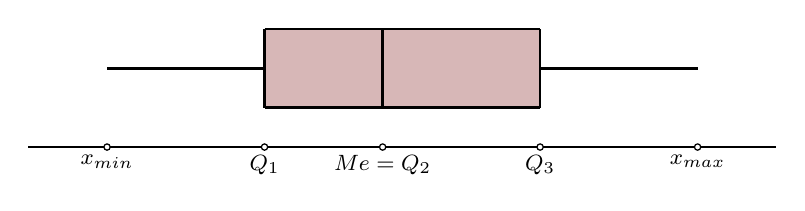
\begin{tikzpicture}
            % \clip (0,0) rectangle (14.000000,10.000000);
            {\footnotesize
            
            % Marking point x_{min} by circle
            \draw [line width=0.016cm] (1.500000,1.000000) circle (0.040000);%
            \draw (1.500000,1.000000) node [anchor=north] { $x_{min}$ };%
            
            % Marking point Q_1 by circle
            \draw [line width=0.016cm] (3.500000,1.000000) circle (0.040000);%
            \draw (3.500000,1.000000) node [anchor=north] { $Q_1$ };%
            
            % Marking point Me=Q_2 by circle
            \draw [line width=0.016cm] (5.000000,1.000000) circle (0.040000);%
            \draw (5.000000,1.000000) node [anchor=north] { $Me=Q_2$ };%
            
            % Marking point Q_3 by circle
            \draw [line width=0.016cm] (7.000000,1.000000) circle (0.040000);%
            \draw (7.000000,1.000000) node [anchor=north] { $Q_3$ };%
            
            % Marking point x_{max} by circle
            \draw [line width=0.016cm] (9.000000,1.000000) circle (0.040000);%
            \draw (9.000000,1.000000) node [anchor=north] { $x_{max}$ };%
            
            % Drawing segment a b
            \draw [line width=0.016cm] (0.500000,1.000000) -- (1.460000,1.000000);%
            \draw [line width=0.016cm] (1.540000,1.000000) -- (3.460000,1.000000);%
            \draw [line width=0.016cm] (3.540000,1.000000) -- (4.960000,1.000000);%
            \draw [line width=0.016cm] (5.040000,1.000000) -- (6.960000,1.000000);%
            \draw [line width=0.016cm] (7.040000,1.000000) -- (8.960000,1.000000);%
            \draw [line width=0.016cm] (9.040000,1.000000) -- (10.000000,1.000000);%
            
            % Changing color 215 183 183
            \definecolor{r215g183b183}{rgb}{0.843137,0.717647,0.717647}%
            \color{r215g183b183}% 
            
            % Filling rectangle left-bottom: f right-top: i
            \fill (3.500000,2.500000) -- (7.000000,2.500000) -- (7.000000,1.500000) -- (3.500000,1.500000);%
            
            % Changing color 0 0 0
            \definecolor{r0g0b0}{rgb}{0.000000,0.000000,0.000000}%
            \color{r0g0b0}% 
            
            % Drawing segment c d
            \draw [line width=0.032cm] (1.500000,2.000000) -- (3.500000,2.000000);%
            
            % Drawing segment e f
            \draw [line width=0.032cm] (3.500000,1.500000) -- (3.500000,2.500000);%
            
            % Drawing segment g h
            \draw [line width=0.032cm] (5.000000,1.500000) -- (5.000000,2.500000);%
            
            % Drawing segment i j
            \draw [line width=0.032cm] (7.000000,1.500000) -- (7.000000,2.500000);%
            
            % Drawing segment k l
            \draw [line width=0.032cm] (7.000000,2.000000) -- (9.000000,2.000000);%
            
            % Drawing segment e i
            \draw [line width=0.032cm] (3.500000,1.500000) -- (7.000000,1.500000);%
            
            % Drawing segment f j
            \draw [line width=0.032cm] (3.500000,2.500000) -- (7.000000,2.500000);%
            \color{black}
            }
            \end{tikzpicture}
        \end{figure}
    

        ~


%%%% naloge


    \begin{naloga}
        Izračunajte aritmetično sredino količin.
        \begin{itemize}
            \item $1.5~s$, $3.5~s$, $1~s$
            \item $4~km$, $2000~m$, $3~km$
            \item $4~€$, $2~€$, $3~€$, $1~€$, $5~€$
        \end{itemize}
    \end{naloga}

    \begin{naloga}
        Izračunajte aritmetično sredino danim podatkom.
        \begin{itemize}
            \item $2, 3, 1, 8, 19, 2, 7$
            \item $13, 39, 12$
            \item $0.3, 0.4, 0.5, 0.7, 0.6$
        \end{itemize}            \end{naloga}



    \begin{naloga}
        Določite modus danim številskim podatkom.
        \begin{itemize}
            \item $1, 4, 2, 4, 1, 6, 3, 4, 1, 4, 6, 4, 4, 8$
            \item $3, 25, 10, 3, 5, 7, 5, 7, 9, 4, 49$
            \item $\dfrac{1}{3}, \dfrac{3}{4}, \dfrac{1}{2}, \dfrac{6}{8}, \dfrac{2}{9}$
            \item $\dfrac{1}{2}, \dfrac{2}{4}, \dfrac{1}{4}, \dfrac{5}{10}, \dfrac{8}{9}$
        \end{itemize}
    \end{naloga}

    \begin{naloga}
        V porodnišnici so izmerili dolžine dojenčkov, ki so se rodili v enem dnevu.  \\
        $50, 51, 51, 44, 47, 48, 53, 49, 52, 55, 46, 50, 50, 49, 47, 47$ \\
        Določite mediano podatkov.
    \end{naloga}





    \begin{naloga}
     
     Otroci v vrtcu so metali žogo na koš in si zapisovali dosežke. Podatki so prikazani v preglednici. 

         \begin{table}[H]
             \centering
             \begin{tabular}{||c|c|c|c|c|c|c|c|c|c||} 
             \hhline{|t:==========:t|}
             \rowcolor[rgb]{0.843,0.718,0.718} 
             Otrok  & Jaka & Jure & Miha & Polona & Valerija & Tina & Mojca & Cene & Darja   \\ 
             \hhline{|:==========:|}
             Št.~košev & $5$ & $7$ & $10$ & $8$ & $5$ & $6$ & $9$ & $9$& $4$  \\ 
             \hhline{|b:==========:b|}
             \end{tabular}
         \end{table}

        Izračunajte, koliko košev je otrok zadel v povprečju. Podatke uredite po vrsti in določite $Mo$, $Me$ ter narišite škatlo z brki.

    \end{naloga}



\end{priprava}
\begin{priprava}{4}{}{Mere razpršenosti}{Osnove statistike}{frontalna, delo v dvojicah/individualno}{drsnice, projekcija, računalniki}

    \section{Mere razpršenosti}

        

            
    Informacijo o \textbf{porazdelitvi} oziroma \textbf{razpršenosti} podatkov lahko izračunamo s pomočjo: 
    variacijskega razmika, interkvartilnega ranga, variance in standarnega odklona.

\subsubsection{Variacijski razmik}
    \textbf{Variacijski razmik} $R$ je razlika med maksimalno in minimalno vrednostjo statistične spremenljivke:
    $$R=x_{max}-x_{min}.$$



    Variacijski razmik je zelo odvisen od ekstremnih vrednosti, posebno osamelcev, 
    zato ga uporabljamo le v kombinaciji z drugimi merami razpršenosti.





\subsubsection{Interkvartilni rang}
    \textbf{Interkvartilni rang} oziroma \textbf{medčetrtinski razmik} $IR$ je razlika med vrednostjo prvega in tretjega kvartila:
    $$IR=Q_3-Q_1.$$

~

    \textbf{Osamelec} je podatek, katerega vrednost je za več kot $3$-kratnik interkvartilnega ranga~$IR$ nad tretjim kvartilom $Q_3$ ali pod prvim kvartilom $Q_1$. \\
    Podatek je ``pogojno osamelec'', če je njegova vrednosz za več kot $1.5$-kratnik interkvartilnega ranga~$IR$ nad tretjim kvartilom $Q_3$ ali pod prvim kvartilom $Q_1$.


~   

    Interkvartilni rang je mera razpršenosti, ki ni občutljiva na osamelce.





\subsubsection{Varianca}
    \textbf{Varianca} $\sigma^2$ predstavlja aritmetično sredino kvadratov odmikov vrednosti statistične spremenljivke od aritmetične sredine:
    $$\sigma^2=\dfrac{(x_1-\overline{x})^2+(x_2-\overline{x})^2+\cdots+(x_n-\overline{x})^2}{N}=\dfrac{1}{N}\sum_{i=1}^n(x_i-\overline{x})^2.$$


% 
%     Večja kot je varianca, bolj so podatki razpršeni.
% 

\subsubsection{Standardni odklon}
    \textbf{Standardni odklon} $\sigma$ izračunamo kot koren variance:
    $$\sigma=\sqrt{\dfrac{(x_1-\overline{x})^2+(x_2-\overline{x})^2+\cdots+(x_n-\overline{x})^2}{N}}=\sqrt{\dfrac{1}{N}\sum_{i=1}^n(x_i-\overline{x})^2}.$$
    Predstavlja povprečje odmikov vrednosti statistične spremenljivke od aritmetične sredine.


~\\~

%%% naloge



\begin{naloga}
 
    V preglednici so predstavljene cene treh izdelkov v trgovini po posameznih mesecih leta 2019. 

     \begin{table}[H]
         \centering
         \begin{tabular}{||c|c|c|c|c|c|c|c|c|c|c|c||} 
         \hhline{|t:============:t|}
         \rowcolor[rgb]{0.843,0.718,0.718} 
         Izdelek  & Jan & Feb & Mar & Apr & Maj & Jun & Jul & Avg & Sep & Okt & Nov    \\ 
         \hhline{|:============:|}
         Kruh  & $3.35$ & $3.29$ & $3.34$ & $3.38$ & $3.38$ & $3.37$ & $3.38$ & $3.55$ & $3.53$ & $3.54$ & $3.49$ \\ 
         \hhline{|:============:|}
         Jagode & $8.73$ & $7.18$ & $5.52$ & $4.48$ & $5.72$ & $5.64$ & $6.49$ & $6.58$ & $7.15$ & $7.58$ & $8.34$ \\ 
         \hhline{|:============:|}
         Cvetača & $2.04$ & $2.17$ & $1.58$ & $1.75$ & $2.13$ & $1.85$ & $1.93$ & $1.87$ & $1.81$ & $1.99$ & $1.80$ \\ 
         \hhline{|b:============:b|}
         \end{tabular}
     \end{table}

     Izračunajte povprečno ceno in standardni odklon cene vsakega izdelka.

 
    \end{naloga}





\begin{naloga}

V preglednici je prikazano število rojstev v Sloveniji po letih. 

 \begin{table}[H]
     \centering
     \begin{tabular}{||c|c|c|c|c|c|c|c|c|c||} 
     \hhline{|t:==========:t|}
     \rowcolor[rgb]{0.843,0.718,0.718} 
     Leto   & $2013$ & $2014$ & $2015$ & $2016$ & $2017$ & $2018$ & $2019$ & $2020$ & $2021$    \\ 
     \hhline{|:==========:|}
     Število  & $21111$ & $21165$ & $20641$ & $20345$ & $20241$ & $19585$ & $19328$ & $18767$ & $18989$ \\ 
     \hhline{|b:==========:b|}
     \end{tabular}
 \end{table}

 Izračunajte povprečno število rojstev in standardni odklon.

\end{naloga}


 \begin{naloga}

    Pridobili smo podatke (urejene po velikosti): $1, 13, 14, 15, 15, 15, 17, 18, 18, 19, 19, 19$, $19, 20$ in $40$.
    \begin{itemize}
        \item Opišite razpršenost podatkov $R$, $IR$, $Q_1$, $Q_3$, $\sigma$, $\overline{x}$.
        \item Največjo in najmanjšo vrednost (v tem primeru sta to osamelca) odstranimo. Kako se spremeni razpršenost podatkov? 
    \end{itemize}
    
\end{naloga}





\end{priprava}
\begin{priprava}{5. 6}{}{Grafično prikazovanje podatkov}{Osnove statistike}{frontalna, delo v dvojicah/individualno}{drsnice, projekcija, računalniki}

    \section{Grafično prikazovanje podatkov}
                

    \subsection*{Strukturni krog}
    
        \textbf{Strukturni krog} ali \textbf{krožni diagram} uporabljamo, kadar so podatki razvrščeni v malo frekvenčnih razredov 
        ali ne dosežejo veliko različnih diskretnih vrednosti.
    
        \begin{figure}[H]
            \includegraphics[scale=0.3]{../../Slike_in_skice/10921.jpg}
            \includegraphics[scale=0.3]{../../Slike_in_skice/1092.jpg}
        \end{figure}

    
        Celoto predstavlja $360^\circ$, za ostale deleže središčne kote izračunamo s sklepnim računom.
    
        ~

    \subsection*{Stolpčni diagram}

        \textbf{Stolpčni diagram} uporabljamo, ko so podatki razvrščeni v veliko frekvenčnih razredov
        ali lahko dosežejo veliko diskretnih vrednosti.
        
        ~
            
        Stolpčni diagrami so lahko \textbf{pokončni} ali \textbf{ležeči}. 
        Če želimo prikazati več podatkov naenkrat, uporabimo \textbf{sestavljeni} ali \textbf{strukturni} stolpčni diagram.
    
        
        \begin{figure}[H]
            \includegraphics[scale=0.3]{../../Slike_in_skice/1093.jpg}
            \includegraphics[scale=0.22]{../../Slike_in_skice/1095.jpg}
            \includegraphics[scale=0.22]{../../Slike_in_skice/1097.jpg} 
            \includegraphics[scale=0.21]{../../Slike_in_skice/1096.jpg}
            
        \end{figure}
    




\newpage

\subsection*{Histogram}

    \textbf{Histogram} uporabljamo za prikaz grupiranih podatkov. 

        \begin{figure}[H]
            \includegraphics[scale=0.33]{../../Slike_in_skice/1098.jpg}
        \end{figure}


    Širine frekvenčnih razredov niso nujno enake.
    Meje razredov narišemo na vodoravni osi, frekvence posameznih razredov pa na navpični osi.



            




~

\subsection*{Linijski diagram}

    \textbf{Linijski diagram/poligon} uporabljamo, ko želimo prikazati postopno spreminjanje vrednosti nekega podatka skozi daljše časovno obdobje.
    Frekvenčne porazdelitve ponazorimo s \textbf{frekvenčnim poligonom}, podatki so lahko zvezni ali grupirani.
        
            \begin{figure}[H]
                \includegraphics[scale=0.23]{../../Slike_in_skice/1166.jpg}
                \includegraphics[scale=0.3]{../../Slike_in_skice/1099.jpg}
            \end{figure}
            

~\\~\\~


%%%% naloge




    \begin{naloga}
 
        Na matematičnem testu je bilo mogoče doseči $50$ točk. Dosežki so bili: 
        $35, 22, 41, 47$, $36, 30, 27, 19, 31, 43, 48, 44, 23, 26, 36, 10, 33, 14, 9$. \\
        Razdelite jih v pet enako velikih razredov ter predstavite s histogramom.
        
    \end{naloga}


    \begin{naloga}
     
     Otroci v vrtcu so metali žogo na koš in si zapisovali dosežke. Podatki so prikazani v preglednici. 

         \begin{table}[H]
             \centering
             \begin{tabular}{||c|c|c|c|c|c|c|c|c|c||} 
             \hhline{|t:==========:t|}
             \rowcolor[rgb]{0.843,0.718,0.718} 
             Otrok  & Jaka & Jure & Miha & Polona & Valerija & Tina & Mojca & Cene & Darja   \\ 
             \hhline{|:==========:|}
             Št.~košev & $5$ & $7$ & $10$ & $8$ & $5$ & $6$ & $9$ & $9$& $4$  \\ 
             \hhline{|b:==========:b|}
             \end{tabular}
         \end{table}

         Izračunajte, koliko košev je otrok zadel v povprečju. Podatke uredite po vrsti in določite $Mo$, $Me$ ter narišite škatlo z brki.

    \end{naloga}





\begin{naloga}
 
    Bojana beleži, koliko časa potrebuje za pot do šole. Podatke je zapisala v preglednico. 

     \begin{table}[H]
         \centering
         \begin{tabular}{||c|c|c|c|c|c|c|c|c|c|c||} 
         \hhline{|t:===========:t|}
         \rowcolor[rgb]{0.843,0.718,0.718} 
         Dan  & 1. & 2. & 3. & 4. & 5. & 6. & 7. & 8. & 9. & 10.   \\ 
         \hhline{|:===========:|}
         Čas [min] & $9$ & $11$ & $10$ & $8$ & $11$ & $10$ & $9$ & $12$& $9$ & $11$ \\ 
         \hhline{|b:===========:b|}
         \end{tabular}
     \end{table}

     S stolpčnim diagramom predstavite, kako pogosto v šolo potuje $8$ minut, $9$ minut ... 

\end{naloga}

\begin{naloga}
 
    V domu ostarelih občanov je $500$ oskrbovancev. Od $50$ do $60$ let jih je $15~\%$, med $60$ in $70$ leti je $160$ oskrbovancev,
    med $70$ in $80$ leti pa $200$ starostnikov. Drugi so stari med $80$ in $90$ let.
    \begin{itemize}
        \item Iz grupiranih podatkov izračunajte povprečno starost oskrbovancev tega doma.
        \item Grafično ponazorite starost oskrbovancev.
    \end{itemize}
    
\end{naloga}




\end{priprava}

\end{document}